\documentclass[../../main.tex]{subfiles}
 
\begin{document}
\label{sec:top}

Radio-frequency (RF) phased arrays have applications in radar telemetry, telecommunications, ground-penetrating radar, scientific instrumentation, and remote sensing \cite{Vieregg_2016,AVVA201746,arnold_2020,PhysRevD.105.122006,10.3390/s21186091,10.1016/j.jappgeo.2022.104876,phased_array_book}.  In the one-dimensional case, $N$ three-dimensional RF antennas are arranged in a line with fixed spacing.  In the two-dimensional case, $N \times M$ three-dimensional antenna elements are arranged in a two-dimensional grid with fixed spacing in both dimensions.  The signal to noise ratio (SNR) of received signals in arrays of dimension $N$ is boosted by a factor of $\approx \sqrt{N}$, because the $N$ signals are combined coherently while thermal background noise adds like $\sqrt{N}$.  The SNR boost is critical for certain kinds of scientific observations.  For example, systems created at the Center for Remote Sensing and Integrated Systems (CReSIS) are flown in polar regions to perform radar sounding of ice sheets for the purposes of geophysics and climate science \cite{arnold_2020}.  Reflected signals carry information about the ice depth, temperature, and internal structure of the ice.  The radio echoes have small SNRs that require phased arrays.  \\ \vspace{2.5mm}

Traditionally, RF phased arrays are designed with commerical computational electromagnetism (CEM) software.  Radio antennas and phased arrays have \textit{radiation patterns} that define directions of maximum transmission power and received sensitivity.  Radiation patterns have a main lobe in which most of the radiation is concentrated, and the angular width of the main lobe is called the beam width.  Other parameters like S-parameters quantify the efficiency of the systems.  CEM packages like XFDTD and HFSS are used to model these properties as a function of frequency \cite{remcom,ansys}.  The XFDTD package, for example, relies on the finite difference time domain (FDTD) method. The FDTD approach is a CEM technique in which spacetime and Maxwell’s equations are broken into discrete form.  Depending on the software license and version, the current price of these products ranges between \$5,000 and \$40,000 USD.  These costs are prohibitive for HSI undergraduate institutions like Whittier College.  Removing this financial barrier to entry would allow diverse undergraduates to study professional RF design. \\ \vspace{2.5mm}

Another drawback of commercial CEM software is the lack of source code access impedes the incorporation of modern machine learning packages.  Phased array properties are determined by the shape of the RF elements and the grid properties of the array.  The parameter space is driven by the complex variety of RF element shapes.  When combined with open-source CEM software, modern machine learning algorithms can locate optimal solutions.  The authors of \cite{10.3390/electronics8121506} review a number of open-source CEM packages.  One interesting choice they describe is the MIT Electromagnetic Equation Propagation (MEEP) package \cite{10.1016/j.cpc.2009.11.008}.  Though MEEP was designed for $\mu$m wavelengths in photonics applications, we have shown that the scale-invariance of Maxwell's equations allows MEEP users to translate designs to wavelengths at the cm-scale.  We have also shown that MEEP can drive the RF phased-array design loop, and that 3D printer schematics can be extracted from this process \cite{electronics10040415,meepcon2022,10.1016/j.cpc.2009.11.008}.  Through this project, diverse undergraduates will gain experience translating machine learning results into a practical solution.  \\ \vspace{2.5mm}

Filament for 3D printers that is conductive in the RF bandwidth is now available commercially.  Funded through an NSF Translational Impact (TI) award (1721644), Multi3D LLC. has produced filament with a resistivity of just $10^{-2} \Omega$ cm: the Electrifi filament.  Several antenna designs have already been produced \cite{8786183,10.1049/iet-map.2017.0104}.  These examples include horn antennas with gain factors of 15 dB at 5.8 GHz, and microstrip patch antennas with gains of 1-2 dB at 2.5 GHz.  The results match expectations from commercial CEM software.  There are, however, virtually no examples of 3D printed RF phased arrays in the [0.1 - 1] GHz bandwidth.  This bandwidth is the most relevant for the aforementioned applications in particle astrophysics and geophysics.  Further, whole new designs can be discovered that improve on designs like the horn and patch antennas by merging machine learning packages with MEEP.  In Sec. \ref{sec:cem}, we review progress already made at Whittier College.  In Sec. \ref{sec:askaryan}, we show how this work enhances the field of UHE-$\nu$ detection.  In Sec. \ref{sec:cresis}, we show how this work enhances the field of radio sounding of ice sheets and ice shelves.  In Sec. \ref{sec:int}, we articulate our vision for the integration of this research into our STEM curriculum.  In Sec. \ref{sec:time_im}, we provide a project timeline, broken into manageable phases.  In Sec. \ref{sec:broad}, we describe the phase of this project designed to help us provide a better education to our students and broader community .

\section{Computational Electromagnetism and Additive Manufacturing}
\label{sec:cem}

In Summer 2020, we received a Faculty Fellowship from the Office of Naval Research (ONR) to design phased arrays in the [0.1 - 5] GHz bandwidth.  This bandwidth is relevant for projects like IceCube Gen2 (radio)\footnote{Whittier College is a member institution of the IceCube Gen2 collaboration.}.  Given our background in the use of RF detectors for UHE-$\nu$ observations in Antarctica (see Sec. \ref{sec:askaryan}), we were qualified to introduce RF phased arrays to our Navy colleagues.  The audience included engineers and programmers that work in acquisition and development for the Naval Surface Warfare Center (NSWC), Corona Division (NSWC Corona).  Our goal was to design a phased array to be integrated as a transmitter in an anechoic chamber that can mimic moving radar echoes.  The facility will serve as a testing facility for active radar systems.  We began by giving lectures on the electromagnetism of phased arrays, with scientific applications.  Our design flow is depicted in Fig. \ref{fig:design}.  To minimize costs and increase undergraduate student access, we decided to investigate open-source CEM options for the design. \\ \vspace{2.5mm}

\begin{figure}
\centering
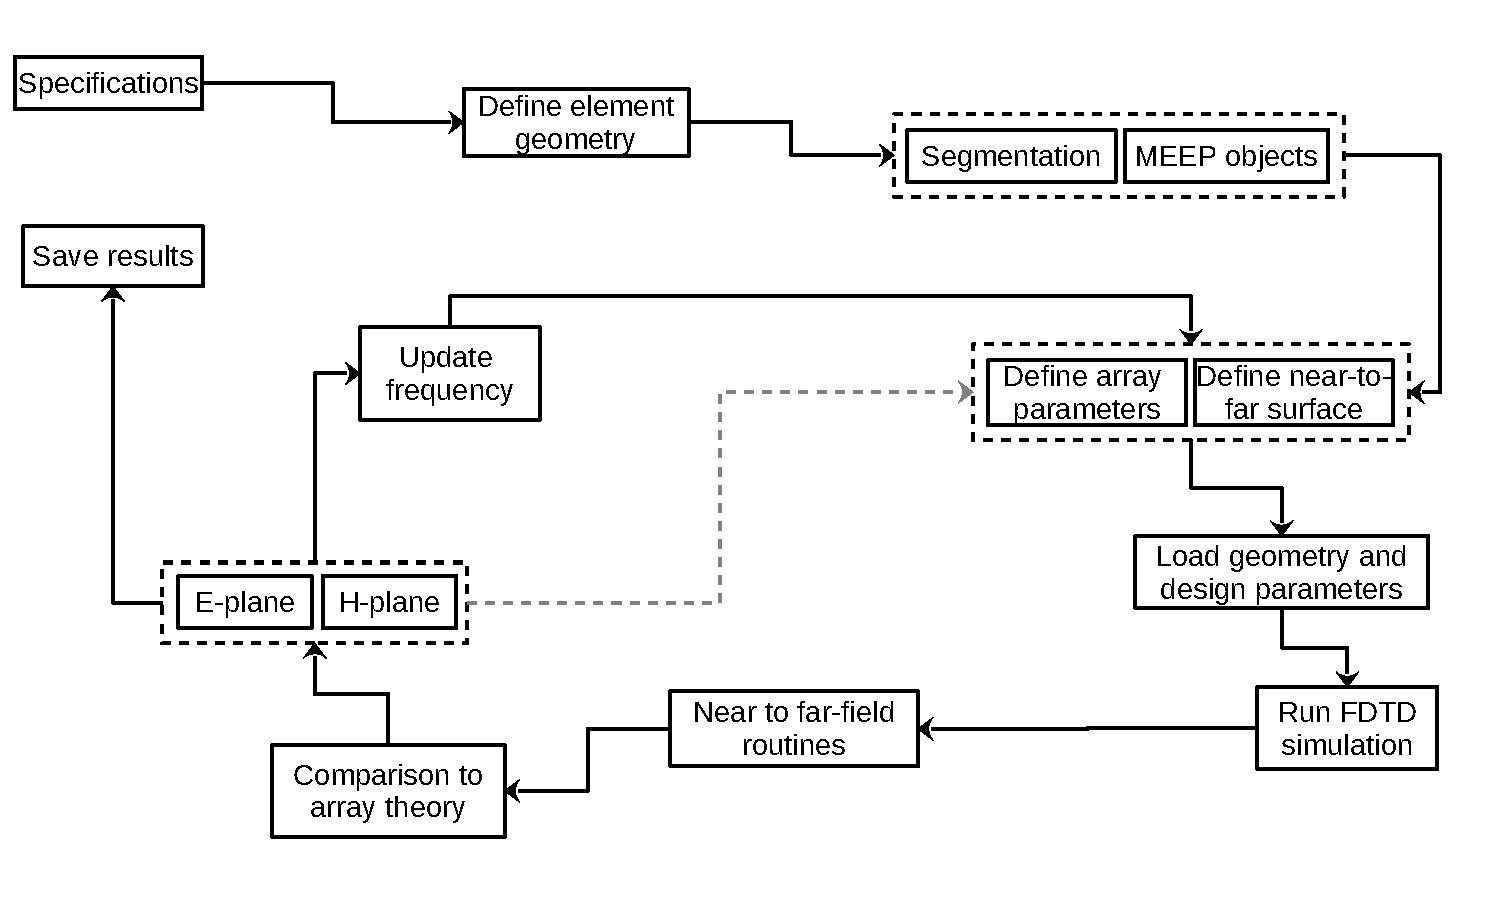
\includegraphics[width=0.85\textwidth]{diagram3.pdf}
\caption{\label{fig:design}  Our design process for RF phased arrays from \cite{electronics10040415}, adapted from Fig. 1 of the review \cite{10.3390/electronics8121506}.}
\end{figure}

We encountered the aforementioned review article in the open-access journal \textit{Electronics} that indicated there are open-source CEM tools that can be adapted to phased array analysis.  Our design flow in Fig. \ref{fig:design} is adapted from Fig. 1 of the review to include specific tasks required for phased arrays, and algorithms for the computation of far-field radiation patterns.  MEEP was noted by the authors in the review as the most advanced among open-source FDTD programs, but they did not benchmark it against HFSS or XFDTD due to the ``steep'' learning curve.  In Summer 2020, we ascended the learning curve and adapted MEEP to RF systems.  A key insight was that MEEP takes advantage of the \textit{scale invariance} of Maxwell's Equations.  The simplest way to understand this is to understand how MEEP uses relative units when discretizing Maxwell's equations for Python code. \\ \vspace{2.5mm}

Like other FDTD methods, MEEP uses a Yee lattice to discretize Maxwell's equations \cite{10.1109/tap.1966.1138693}.  When the speed of light is set to unity ($c = 1$), distance and time units become the same.  Frequency and wavelength units are the inverse of each other.  But distance and wavelength can take \textit{any} unit of length in the Yee lattice.  Most MEEP users interpret this unit of length to be 1 $\mu$m for photonics applications.  For example, a \textit{relative} frequency (unit-less) of 0.5 corresponds to a \textit{relative} wavelength of 2.  When interpreted as 2 $\mu$m, the frequency is 150 THz in real units in the optical bandwidth.  Interpreted as 2 cm, the real frequency is 15 GHz.  A \textit{relative} frequency of 0.05 corresponds to the RF frequency 1.5 GHz.  Assuming design components have sufficient conductivity at RF frequencies, we have re-purposed MEEP as an RF simulator.  \\ \vspace{2.5mm}

\begin{figure}[ht]
\centering
%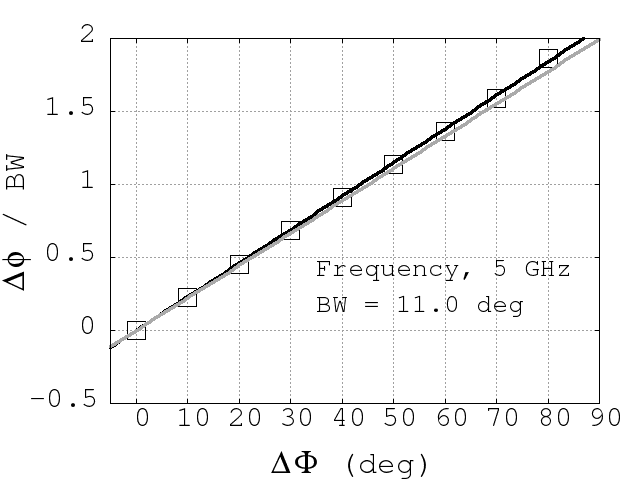
\includegraphics[width=0.35\textwidth]{figures/Oct30_plot2.png}
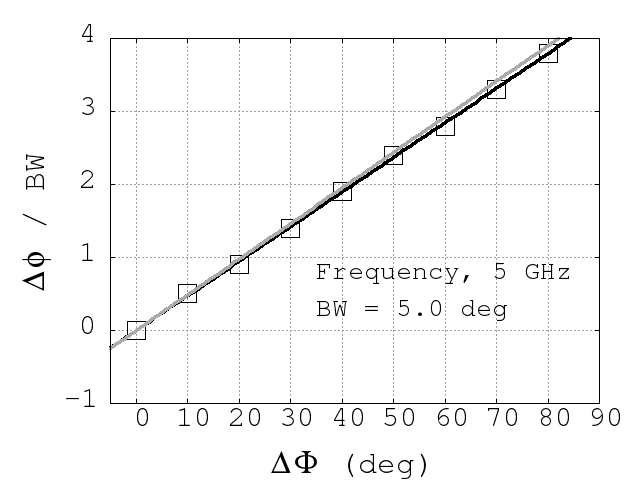
\includegraphics[width=0.33\textwidth]{figures/Oct30_plot1.png}
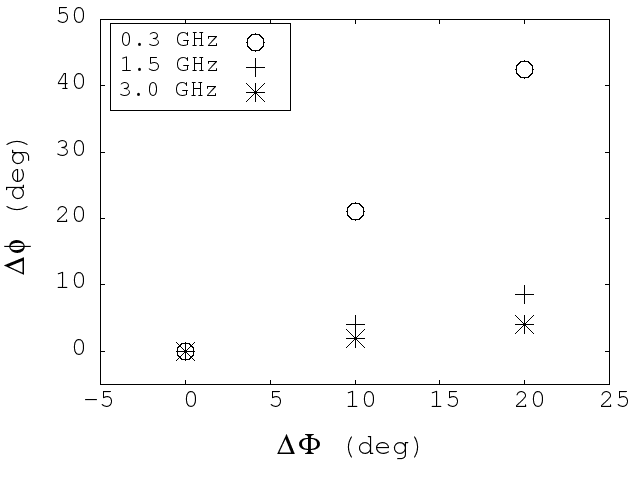
\includegraphics[width=0.33\textwidth]{figures/Aug11_plot2.png}
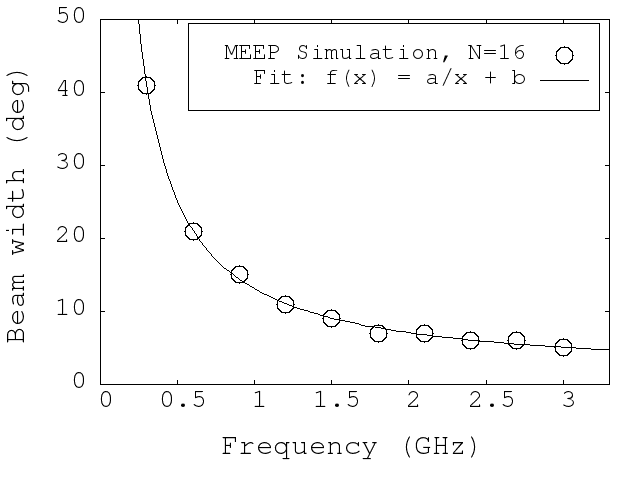
\includegraphics[width=0.33\textwidth]{figures/Aug11_plot1.png}
\caption{\label{fig:pa_1} (Left) The beam angle $\Delta \phi$ divided by the beam width $BW$ for the $N = 16$ one-dimensional Yagi array versus $\Delta \Phi$, the phase shift per element. The gray line represents theoretical expectation, and the black line is a linear fit to the data.  (Middle) $\Delta \phi$ versus $\Delta \Phi$ for the $N=16$ version of the one-dimensional horn array, for several frequencies.  (Right) The dependence of the beam width on frequency for the one-dimensional $N=16$ horn array.  The black line is a functional fit to the data $f(x) = a/x + b$ with $a=12.0\pm 0.1$ degree GHz, and $b=1.1\pm 0.2$ degrees.}
\end{figure}

By Fall 2020, we were producing CEM models using MEEP that matched expected phased array properties.  For a one-dimensional array with $N$ elements, there is a linear relationship between the radiated plane-wave direction $\Delta \phi$, and the phase shift per element $\Delta \Phi$.  The $\Delta \phi$ is also called the \textit{beam angle}.  Figure \ref{fig:pa_1} contains results for our first phased array models in which the elements were Yagi-Uda antennas and horn antennas.  The linear relationship between $\Delta \phi$ and $\Delta \Phi$ is evident in the data.  The $\Delta \phi$ is divided by the beam width (BW) in Fig. \ref{fig:pa_1} (left), and is left in degrees in Fig. \ref{fig:pa_1} (middle).  In Fig. \ref{fig:pa_1} (left), the single-frequency $N=16$ Yagi array can steer a 5 GHz plane wave up to four beam widths to the right or left of the forward direction.  In Fig. \ref{fig:pa_1} (middle), results are shown for an $N=16$ array of horn antennas.  Unlike the Yagi-Uda, the horns are broadband radiators.  Thus, the linear relationship is shown for 0.3, 1.5, and 3.0 GHz.  The beam width is not constant, so $\Delta \phi$ was left in degrees in Fig. \ref{fig:pa_1} (middle).  In Fig. \ref{fig:pa_1} (right), the inverse relationship between beam width and frequency is shown. \\ \vspace{2.5mm}

We also produce CEM phased array radiation patterns that match array theory.  The pattern of a phased array can be derived from first principles \cite{electronics10040415}.  The \textit{pattern multiplication theorem} states that the radiation pattern of a phased array of $N$ identical elements will be that of a row of $N$ point sources, multiplied by the radiation pattern of the element.  In Fig. \ref{fig:1dhornresults2} (left and middle), the radiated E-field of a $N=16$ horn array is shown in the E-plane (x-y plane).  The radiation pattern is represented by the blue curve in Fig. \ref{fig:1dhornresults2} (right).  The beam angle of the main lobe is $\Delta \phi = 9$ degrees above the x-axis, matching the theoretical expectation in red.  The red curve corresponds to the formula for a row of $N$ point sources, which has a back lobe at $\Delta \phi = 171$ degrees due to symmetry.  The horn array has no back lobe because the individual horns suppress it, as expected from the pattern multiplication theorem.  Like the theoretical expectation, the CEM pattern has \textit{side lobes} around the main lobe ($\approx -15$ dB).  We achieved similar results for two-dimensional arrays of Yagi-Uda and horns.  Our revelation that MEEP could be used to design RF phased arrays earned the article Top 10 honors for December 2020 - May 2021 from the editors of \textit{Electronics}. \\ \vspace{2.5mm}

\begin{figure}[ht]
\centering
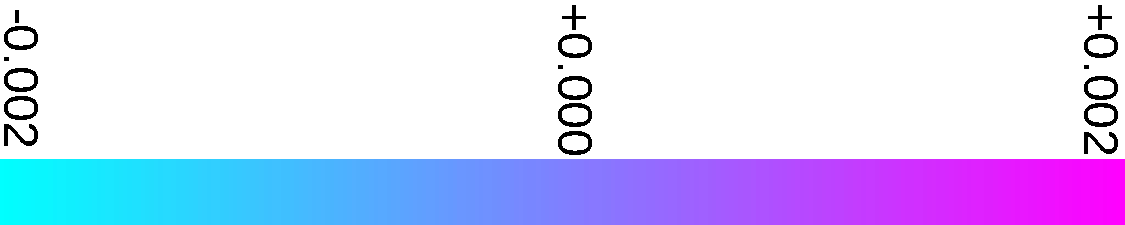
\includegraphics[width=5.625cm,angle=90]{figures/fields/colorbar.pdf}
%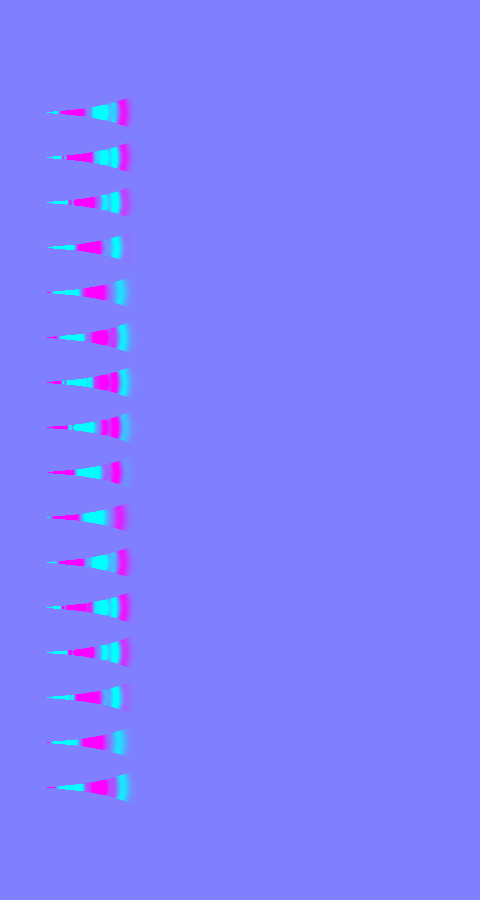
\includegraphics[width=3cm]{figures/fields/ey_phase_horn_t15.png}
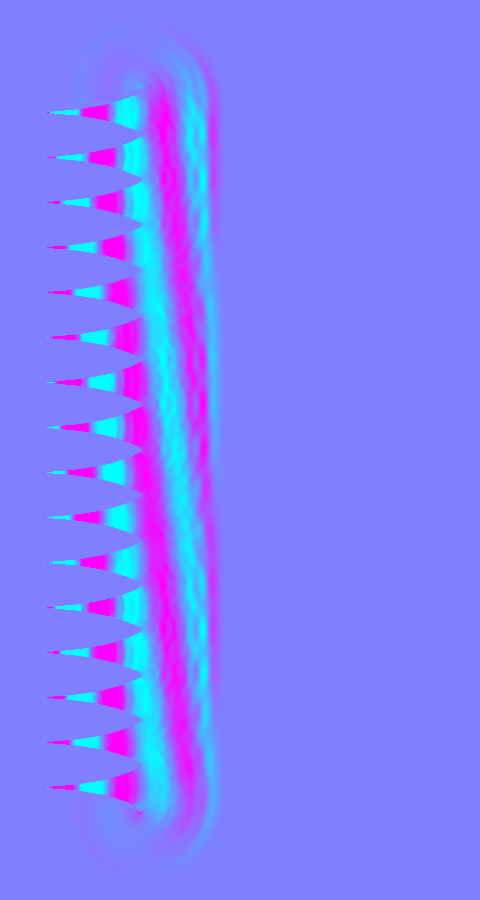
\includegraphics[width=3cm]{figures/fields/ey_phase_horn_t30.png}
%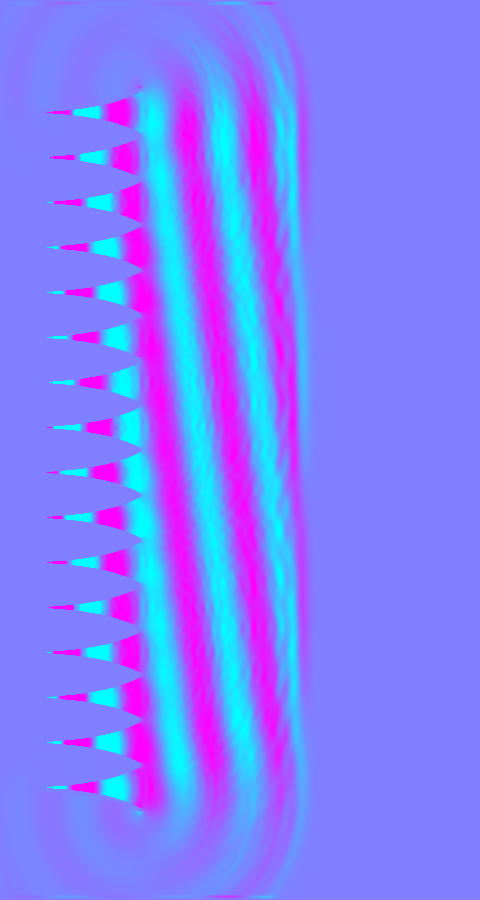
\includegraphics[width=3cm]{figures/fields/ey_phase_horn_t45.png}
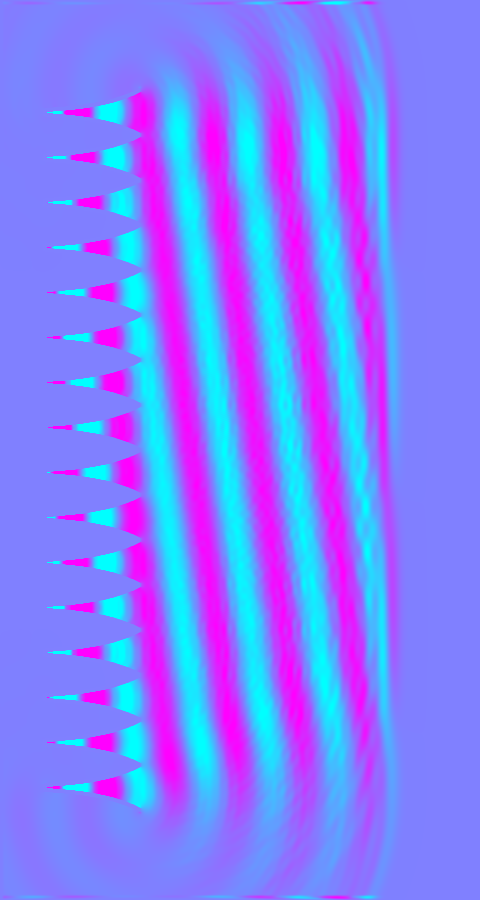
\includegraphics[width=3cm]{figures/fields/ey_phase_horn_t60.png}
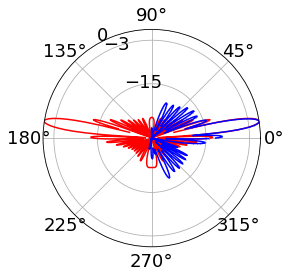
\includegraphics[width=6cm]{figures/fields/rad_patt_field.png}
\caption{\label{fig:1dhornresults2} (Left) The $N = 16$ horn array, radiating the linearly polarized $\vec{E}(x,y,t)$ (y-component shown, in arbitrary units) at $t = 1$ ns into the simulation run, and (middle) at $t = 2$ ns into the run.  The 2D area is $80 \times 150$ cm$^2$.  The frequency is 2.5 GHz, and the beam angle is $\Delta \phi = 9$ degrees above the x-axis. (Right) The normalized radiated power in dB versus $\Delta \phi$ in degrees.  The blue curve represents the results from MEEP, and the red curve is the theoretical expectation from $N$ point sources.}
\end{figure}

\begin{figure}[hb]
\centering
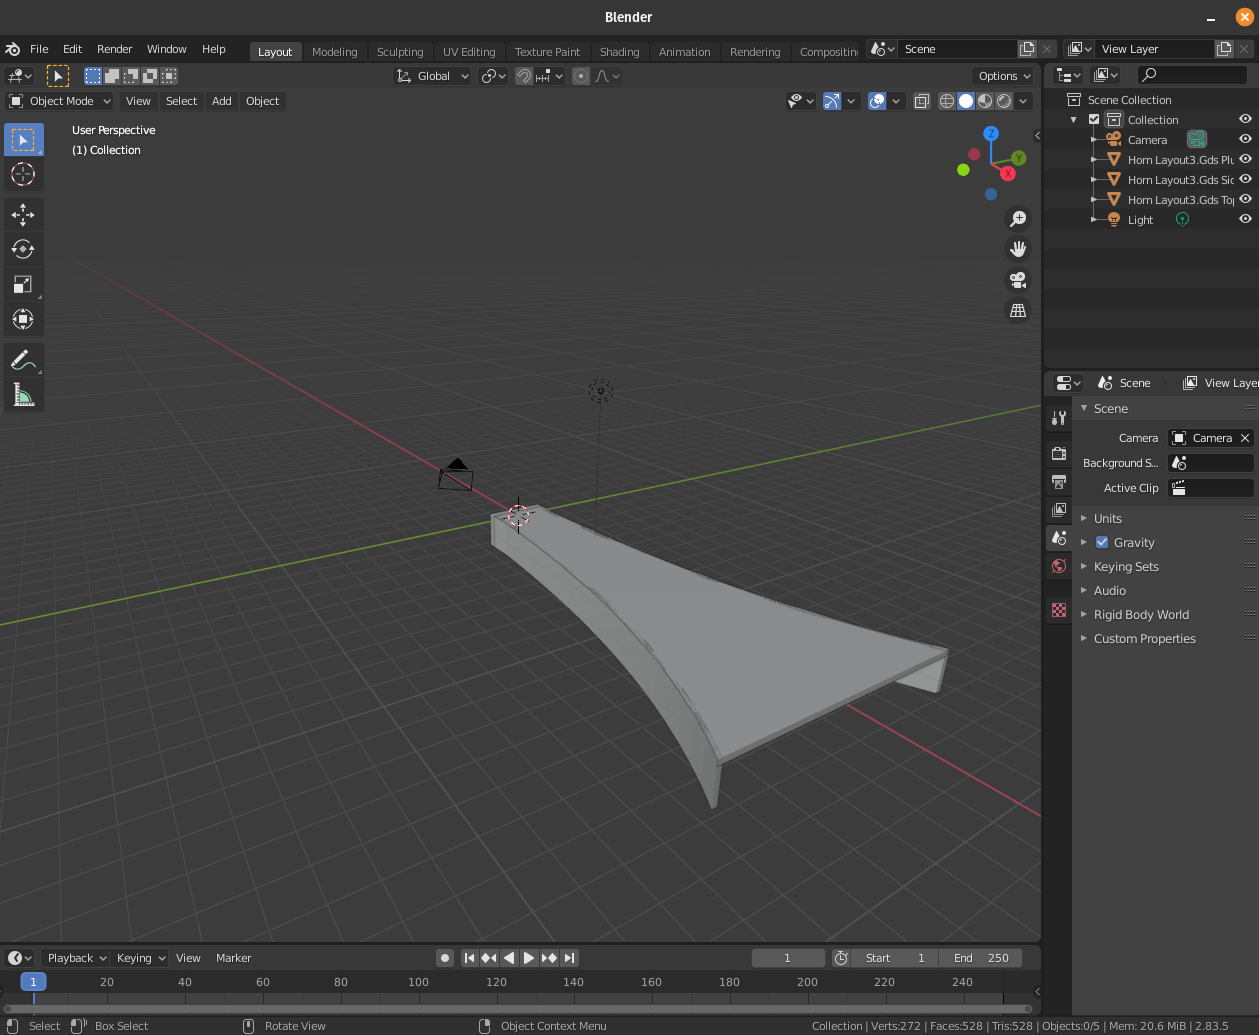
\includegraphics[width=0.4\textwidth]{figures/blender_example.png}
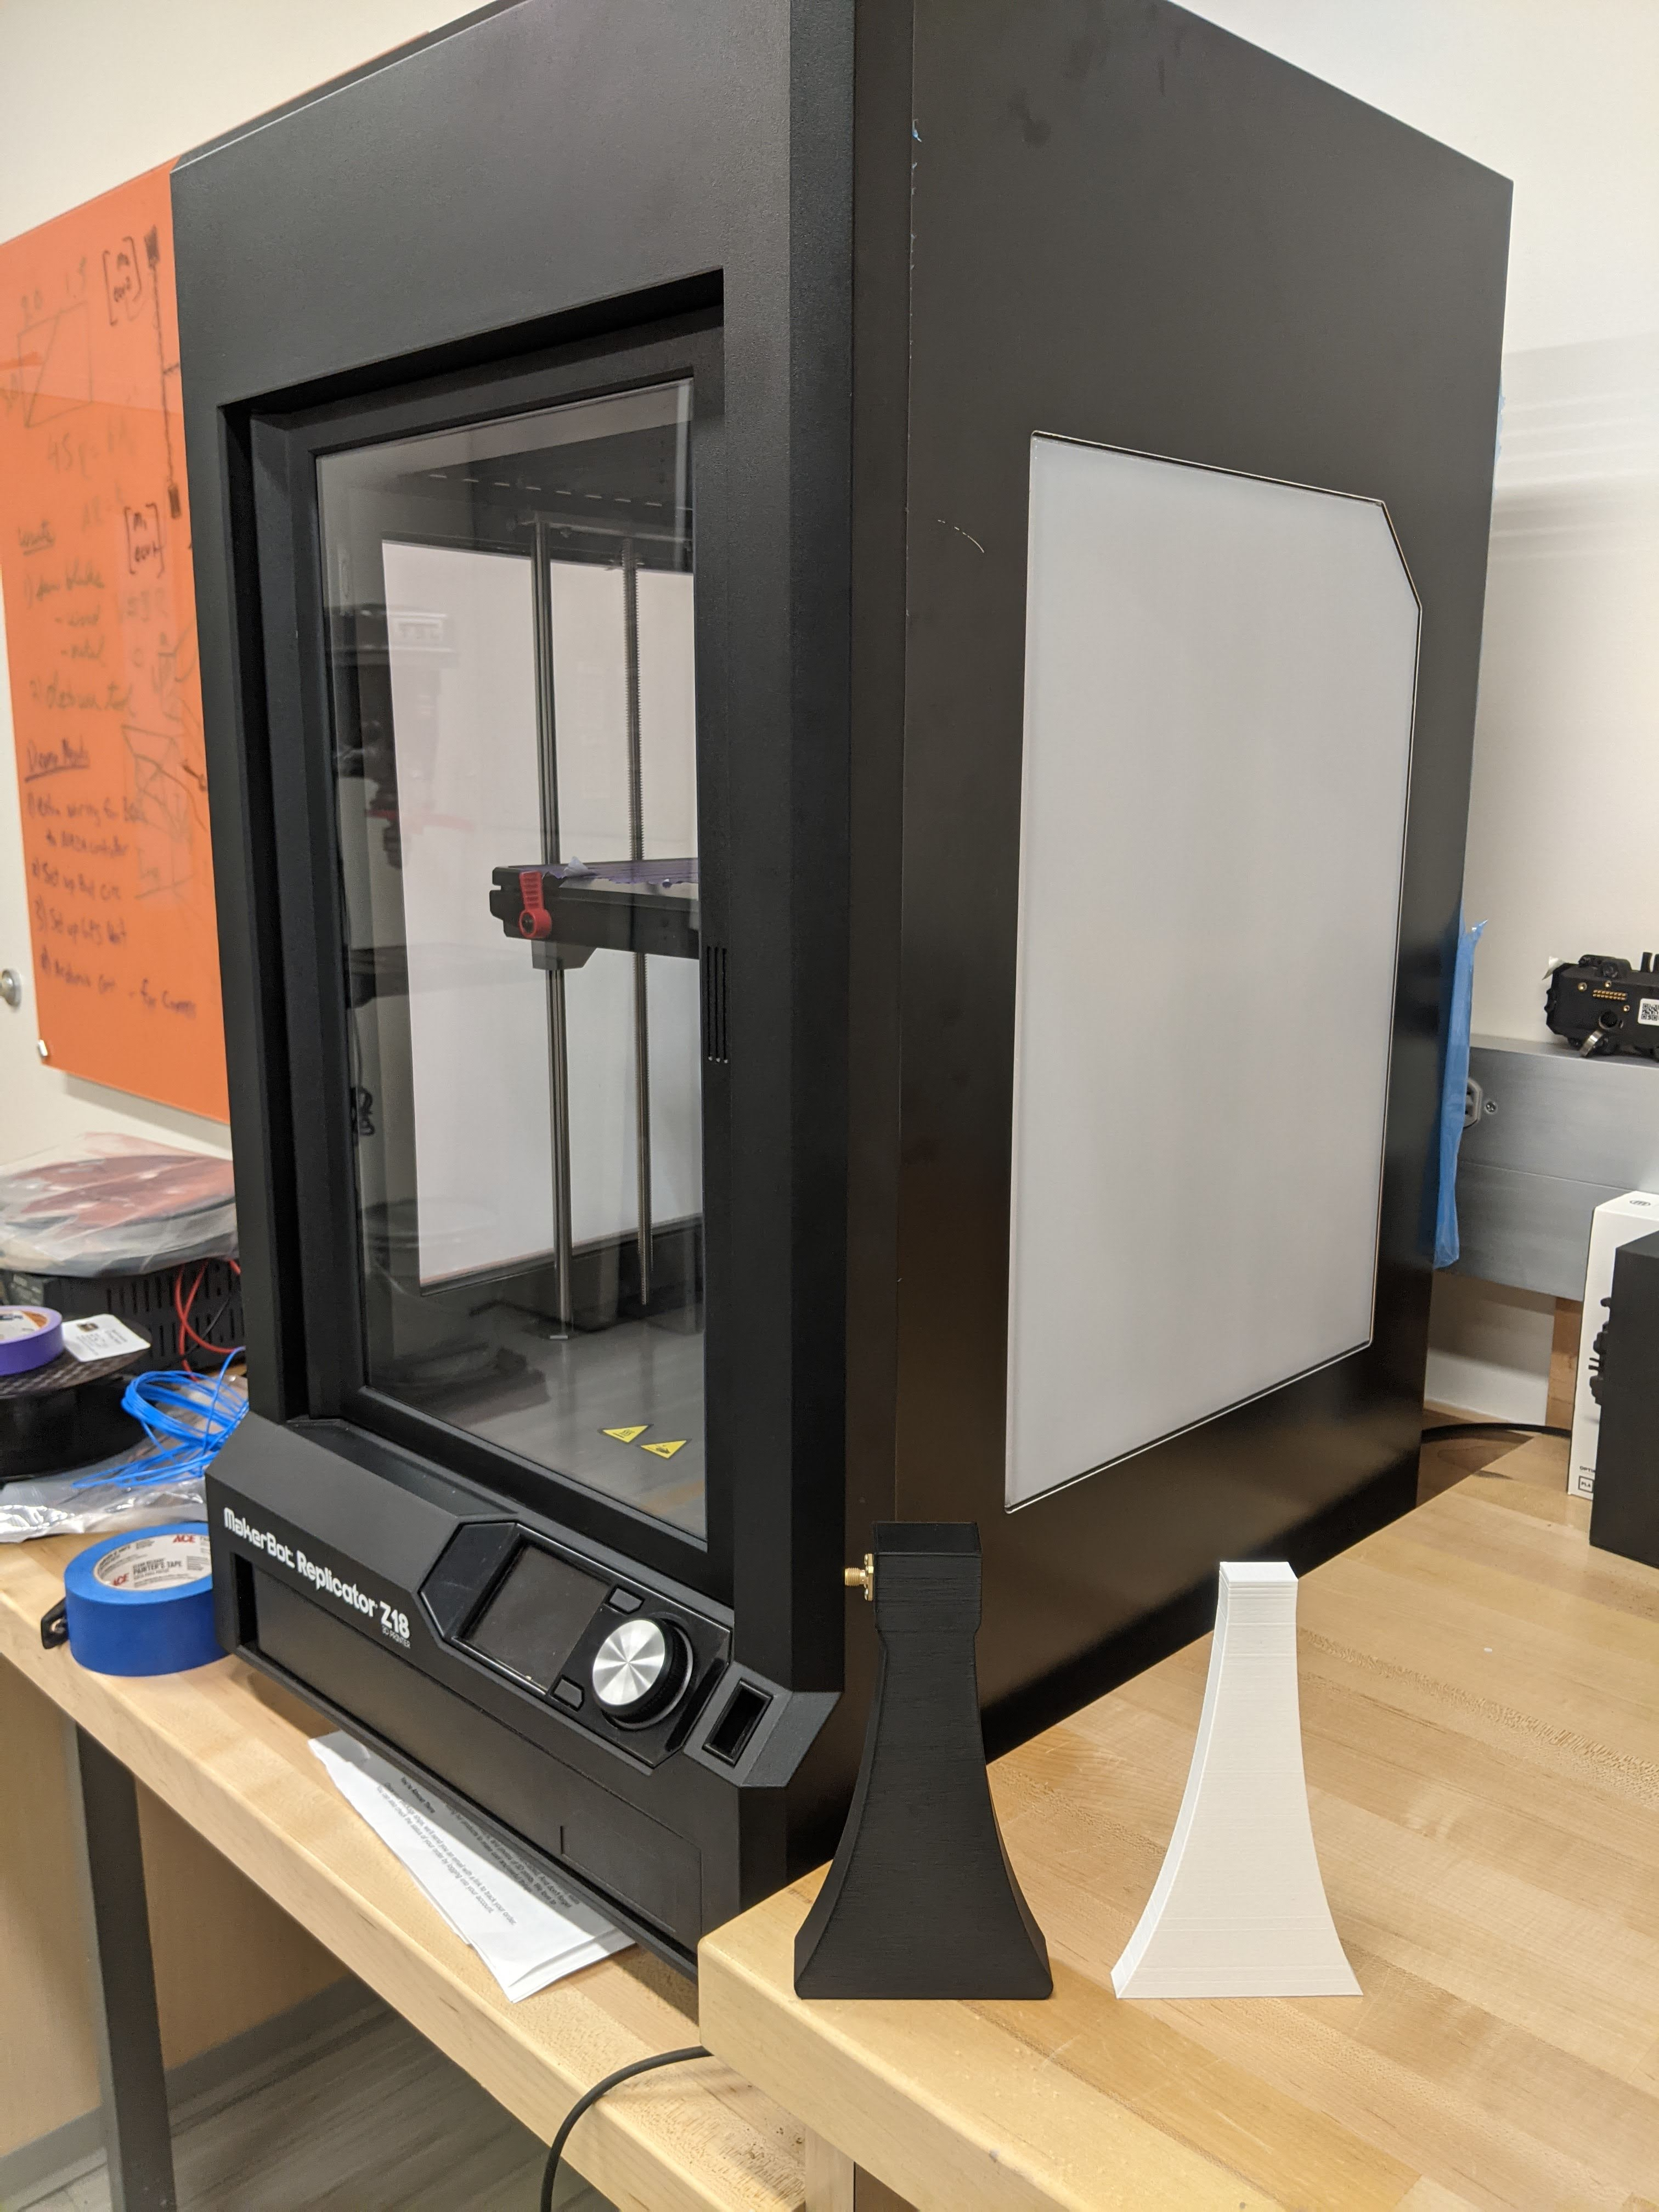
\includegraphics[width=0.2\textwidth]{figures/3dprinter.jpg}
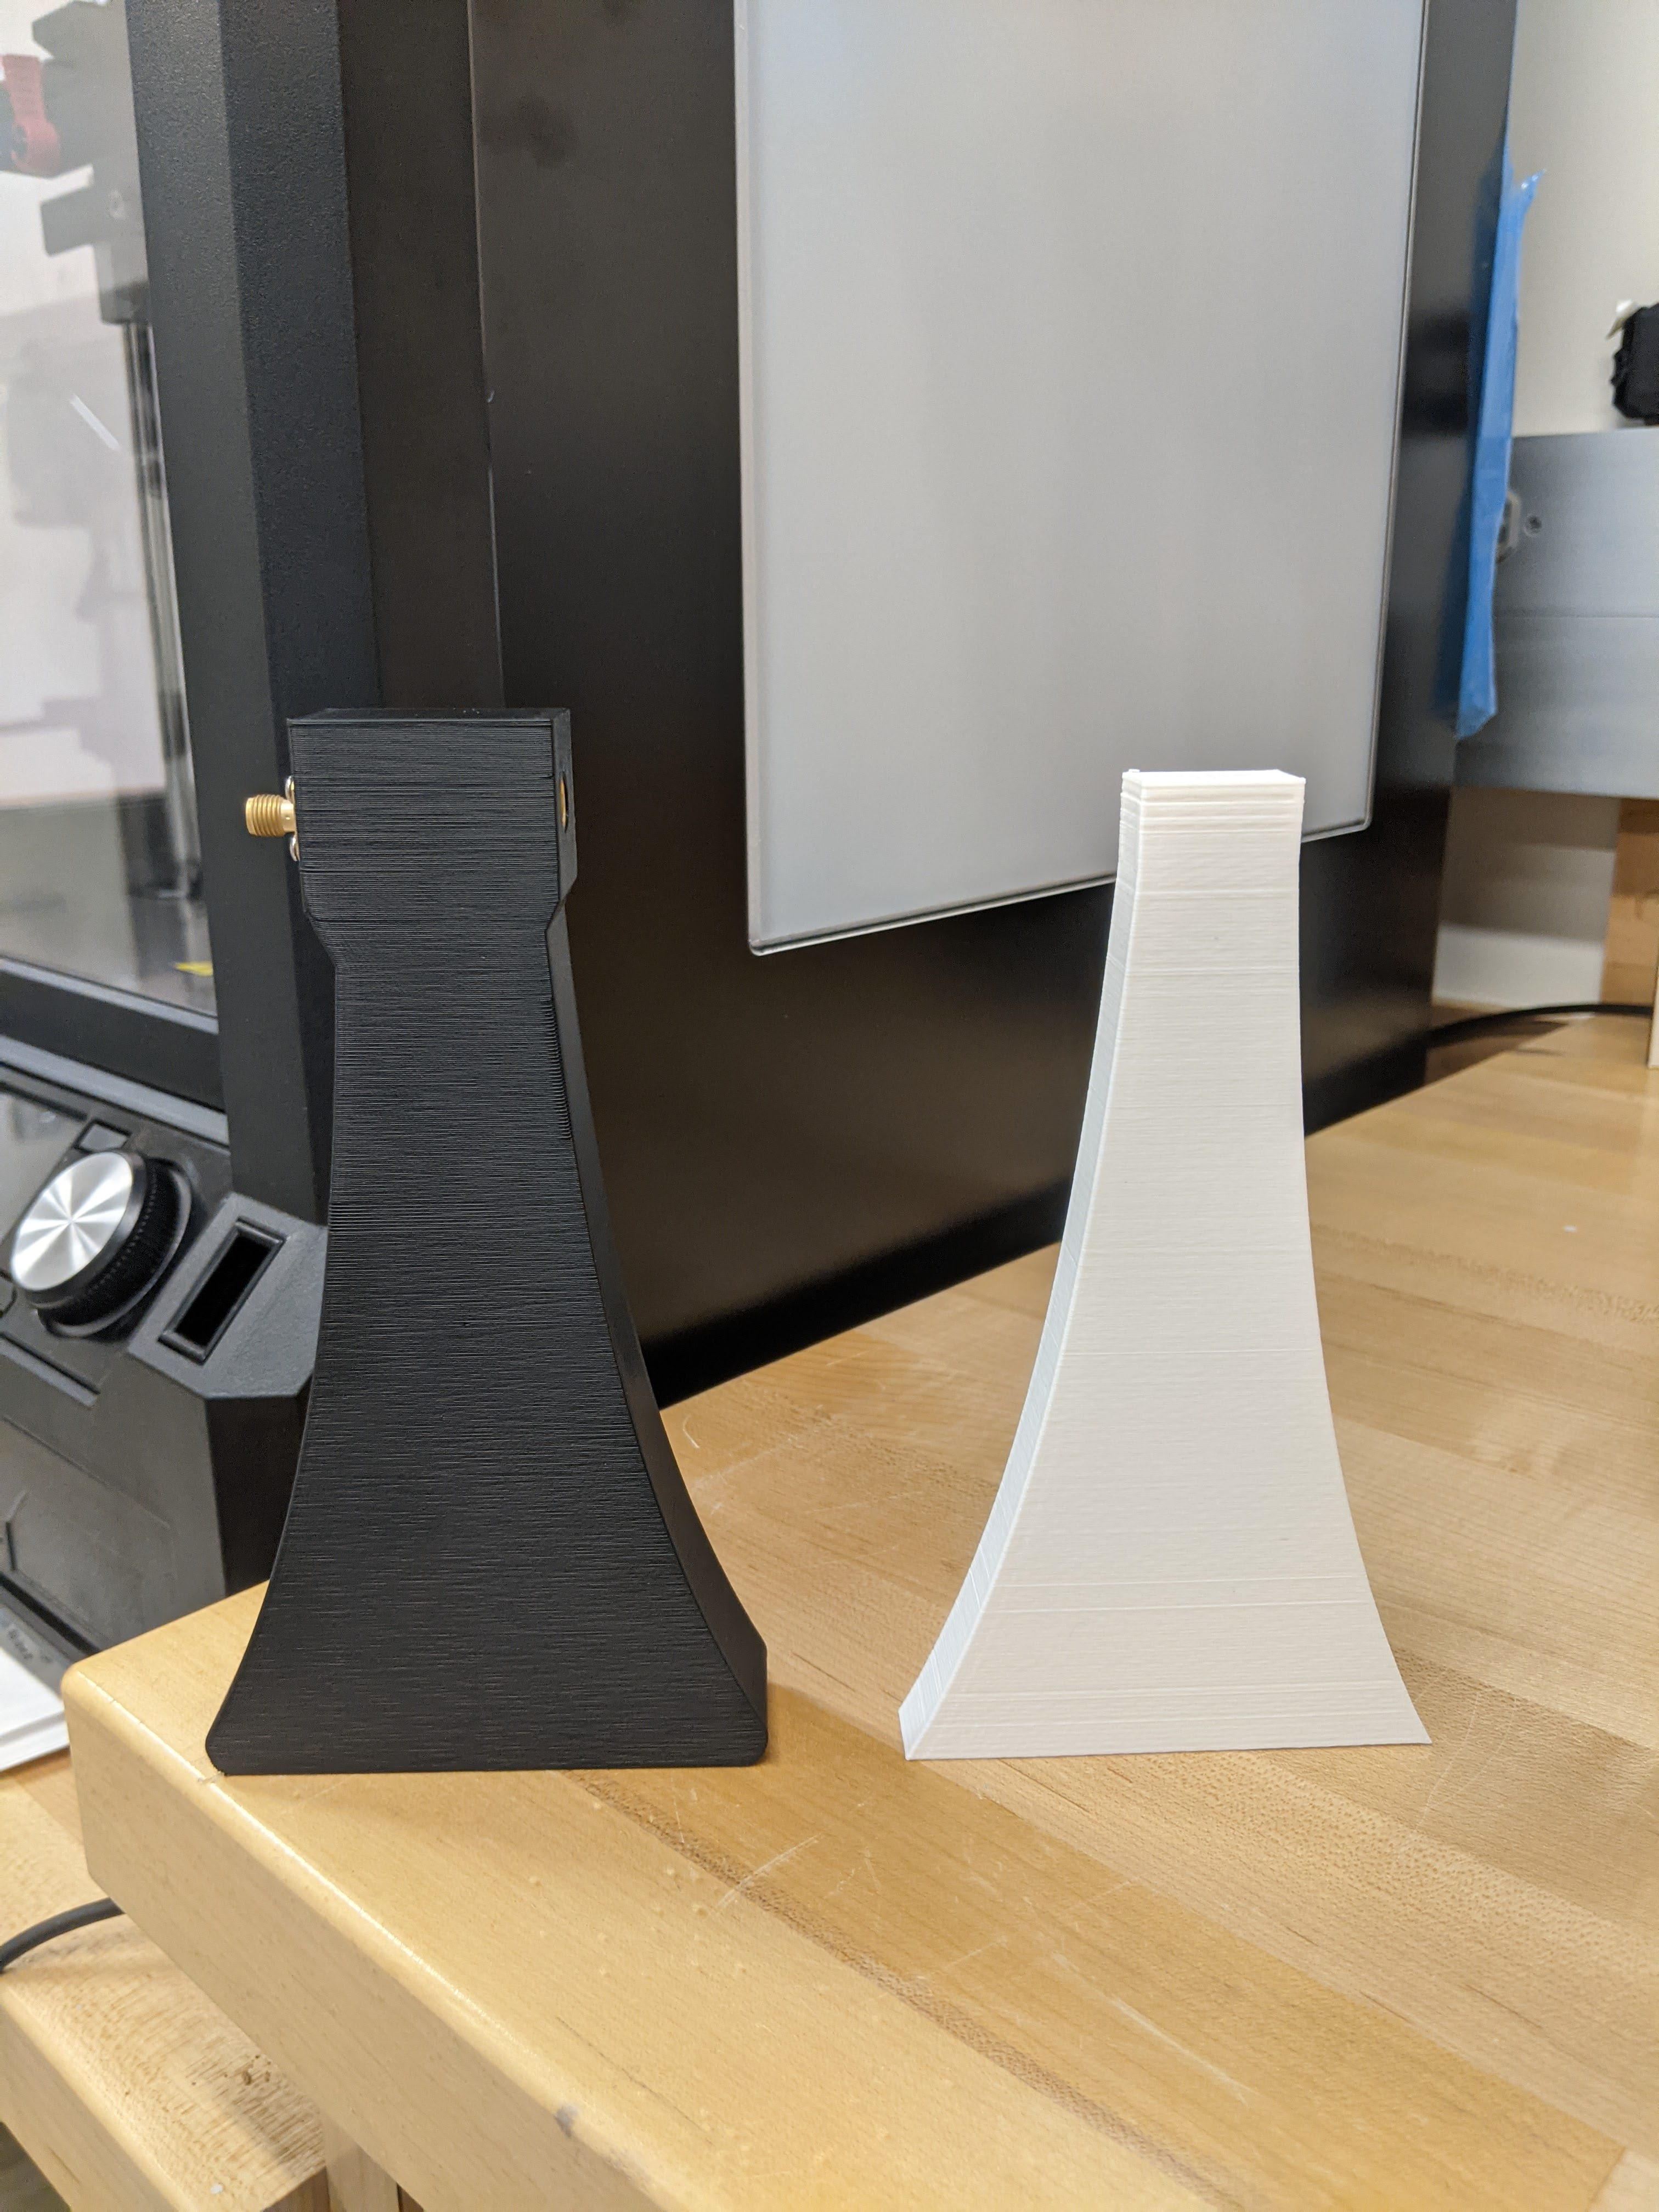
\includegraphics[width=0.2\textwidth]{figures/3dprinter_2.jpg}
\caption{\label{fig:3d_print} (Left) Blender/STL files extracted from MEEP code.  (Middle) MakerBot 3D printer, with PLA horn model (white), and  proto-pasta with SMA connector (black). (Right) Close-up of horns.}
\end{figure}

In Summer 2021, we received a second ONR fellowship to continue the research.  We determined how to integrate CAD design with MEEP in 2D, and later 3D.  As a result, we can now simulate the radiation patterns and S-parameters of the exact object we hope to print.  We acquired NinjaTek proto-pasta 3D printer filament, advertised as conductive.  We printed a horn with in-built SMA connecter for RF cables (Fig. \ref{fig:3d_print}).  The proto-pasta result had a measured resistance of $\approx 10$ k$\Omega$, too large for an RF antenna.  Multi3D LLC, the manufacturer of the Electrifi filament, has now provided resistivity results that compare proto-pasta with Electrifi (Fig. \ref{fig:3d_print2}).  The Electrifi filament will improve resistivity by two orders of magnitude.  We seek to print Electrifi-based antennas, and to measure the radiation pattern and S-parameters. \\ \vspace{2.5mm}

\begin{figure}[ht]
\centering
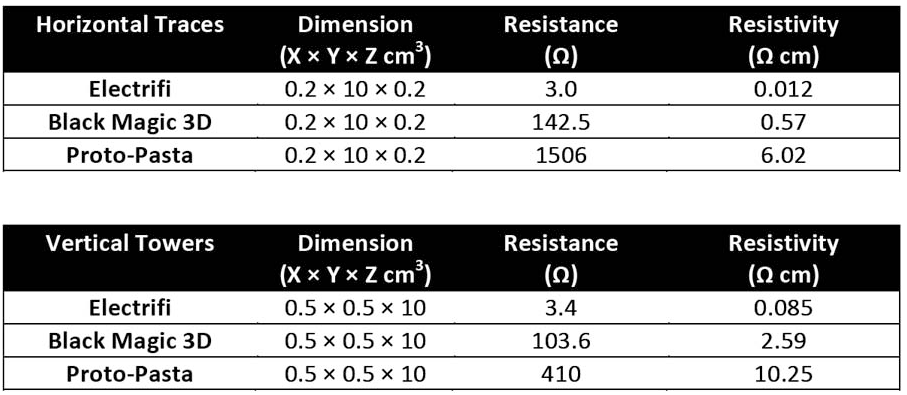
\includegraphics[width=0.65\textwidth]{figures/multi3dllc.png}
\caption{\label{fig:3d_print2} Resistivity results published by Multi3D LLC that compare the proto-pasta product with the new Electrifi conductive filament (\url{https://www.multi3dllc.com/faqs/}).}
\end{figure}

In Summer 2022, we received a final ONR fellowship focusing on GPS modernization.  Alongside this work, we continued to refine the open-source CEM results.  We learned to simulate the full 3D horns stored in CAD files using parallel processing, achieving an order of magnitude reduction in computation time.  The results are shown in Fig. \ref{fig:3d_cad}.  In Fig. \ref{fig:3d_cad} (a), the main lobes are designed to point to 0 degrees (x-direction) for the E-plane (x-y plane), and 90 degrees for the H-plane (x-z plane).  The E-plane contains the linearly polarized radiation vector.  In Fig. \ref{fig:3d_cad} (b), the (voltage standing wave ratio) VSWR is shown.  The VSWR is a common figure of merit for RF antennas, related to the S-parameters.  The VSWR approaches 1 for an efficiently radiating antenna, and infinity for no efficiency.  The radiation patterns match expectations for horn antennas (see Fig. 19 of \cite{8786183}).  The VSWR results demonstrate efficient radiation in the bandwidth [0.5 - 6] GHz.  We presented our progress at the annual MeepCon 2022 at the Massachusetts Institute of Technology (MIT) \cite{meepcon2022}.  We learned new techniques for integrating MEEP and machine learning tools \cite{meepcon2022_2}, and how eager MEEP developers are to collaborate in the RF regime.  \\ \vspace{2.5mm}

\begin{figure}[ht]
\centering
\begin{subfigure}{0.65\textwidth}
    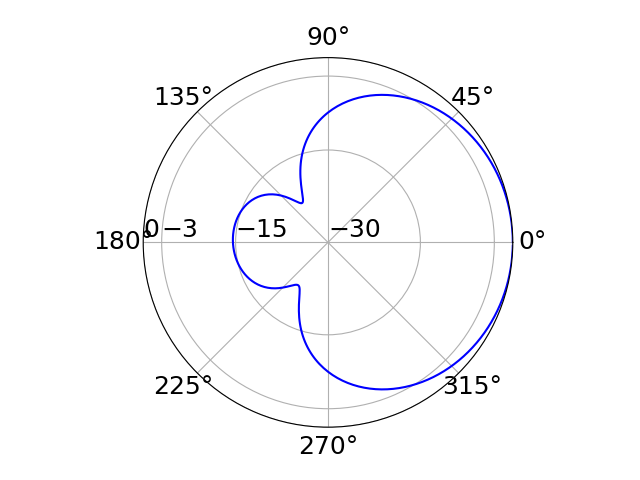
\includegraphics[width=0.49\textwidth]{figures/3DHorn_CAD_0_5GHz_E_plane.png}
	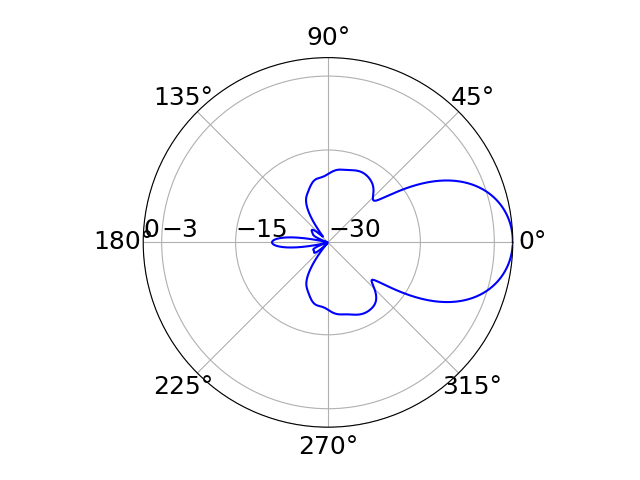
\includegraphics[width=0.49\textwidth]{figures/3DHorn_CAD_5GHz_E_plane.png} \\
	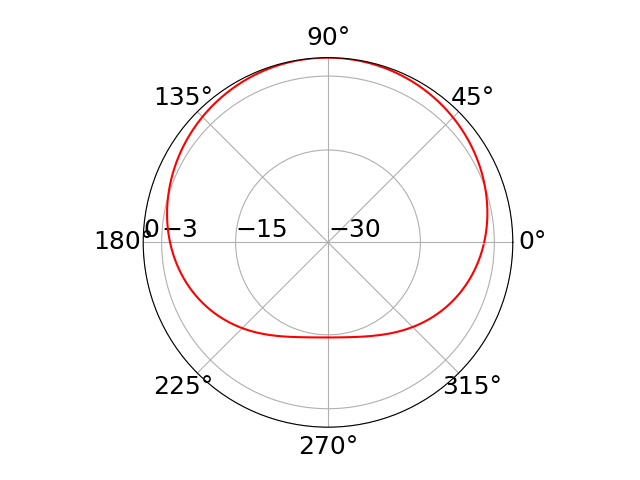
\includegraphics[width=0.49\textwidth]{figures/3DHorn_CAD_0_5GHz_H_plane.png}
	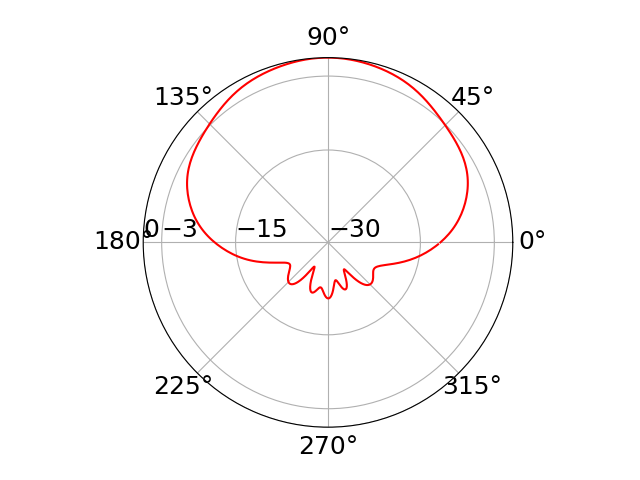
\includegraphics[width=0.49\textwidth]{figures/3DHorn_CAD_5GHz_H_plane.png}
    \caption{Radiation pattern results using GDSII/CAD for (top left) E-plane at 0.5 GHz, (top right) E-plane at 5.0 GHz, (bottom left) H-plane at 0.5 GHz, (bottom right) H-plane at 5.0 GHz.  See text for details.}
\end{subfigure}
\hfill
\begin{subfigure}{0.3\textwidth}
    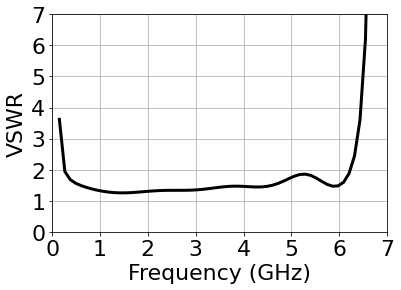
\includegraphics[width=0.99\textwidth]{figures/vswr.png}
	\caption{The VSWR figure of merit versus frequency in GHz for the RF horn.}
\end{subfigure}
\caption{Results for RF horn design, using the open-source design process open to 3D printing.}
\label{fig:3d_cad}
\end{figure}

\subsection{RF Laboratory Capability and Prior ONR Funding}

We are required to take a research gap year in Summer 2023, according to ONR regulations.  However, we have now begun an Educational Partnership Agreement (EPA) between NSWC Corona and Whittier College.  NSWC Corona now has the ability to transfer laboratory equipment to Whittier College.  NSWC Corona has provided RF bench testing equipment that is perfectly suited to the proposed work.  A list of instruments transferred from NSWC Corona between 2020 and 2023 is shown in Tab. \ref{tab:equip}.  Our network analyzer and power sensors can perform S-parameter measurements over [0.1 - 5 GHz] for our antennas under test (AUT).  Our signal generator can create calibration signals for our calibration antennas and AUT in the proposed bandwidth.  Our calibration antennas serve as benchmark devices for comparison to our 3D printed AUT.  Due to the precision and wide bandwith of these devices, regular calibration is required.  Our calibration kits serve this purpose.  Our laboratory is therefore well-equipped to complete the proposed work, and this minimizes budgetary impact. \\ \vspace{2.5mm}

This research has been completed with significant contributions from diverse undergraduate students.  We provide a summary of funding for personnel that have contributed to the early stages of this work in Tab. \ref{tab:funds}.  These researchers have diverse majors and interests, including our 3-2 Engineering Program (Wildanger), Physics and Math double major (Hartig), and Math/Integrated Computer Science (G\'{o}mez-Reed) and Householder), and Physics and Astronomy (Goodman and Smith).   After Whittier College, these students have begun science and engineering roles that include the Laser Interferometric Gravitation Observatory (LIGO), the University of Southern California (USC), and The Aerospace Corporation.  Whittier College has a good track record of providing access to higher education, and careers in science and technology, to diverse students from Los Angeles County and beyond. \\ \vspace{2.5mm}

\begin{table}
\centering
\begin{tabular}{c c c}
Equipment & Bandwidth & Cost \\ \hline
Rohde and Schwartz ZVL6 Network Analyzer & 9 kHz to 6 GHz & \$20k \\
Rohde and Schwartz NRP-91 Power Sensors (2) & 9 kHz to 6 GHz & \$8k \\
Aeroflex 3416 Digital RF Signal Generator & 250kHz to 6 GHz & \$12k \\
Calibration antenna kits (2) & Varies by antenna & \$2k \\
Calibration test kits for Network Analyzer (2) & 6 kHz to 9 GHz & \$6k
\end{tabular}
\caption{\label{tab:equip} A listing of the equipment provided to our labs by the Office of Naval Research.}
\end{table}

\begin{table}
\centering
\begin{tabular}{c c c c}
Student/Professor & Grant Opportunity & Amount & Dates \\ \hline
Jordan C. Hanson & ONR Summer Faculty Fellow & \$16.5k & Summer 2022 \\
Dane Goodman & Summer researcher & Course credit & Summer 2022 \\
Andrew Householder & Summer researcher & Course credit & Summer 2022 \\
Raymond Hartig & Ondrasik-Groce Fellowship & \$5k & Summer 2022 \\
Jordan C. Hanson & ONR Summer Faculty Fellow & \$16.5k & Summer 2021 \\
Adam Wildanger & Fletcher Jones Fellowship & \$5k & Summer 2021 \\
Jordan C. Hanson & ONR Summer Faculty Fellow & \$16.5k & Summer 2020 \\
Raymond Hartig & Fletcher Jones Fellowship & \$5k & Summer 2020 \\
John Paul G\'{o}mez-Reed & Ondrasik-Groce Fellowship & \$7.5k & Summer-Fall 2019 \\
John Paul G\'{o}mez-Reed & Keck Fellowship & \$5k & Summer 2018 \\
Cassady Smith & Keck Fellowship & \$5k & Summer 2018 \\
\end{tabular}
\caption{\label{tab:funds} A listing of the grant opportunities awarded to our group for RF design, softrware development, and machine-learning.  All students are at the undergraduate level.}
\end{table}


\section{The Connection to Ultra-High Energy Neutrino Observations}
\label{sec:askaryan}

The flux of neutrinos with energies between [0.01-1] PeV ($10^{15}$ eV) has been detected by IceCube \cite{10.1126/science.1242856}.  The UHE-$\nu$ flux, with energies above 1 PeV, could explain the unknown origin of UHE cosmic rays (UHECR) \cite{Ackermann:201946d}.  This flux also represents an opportunity to study electroweak interactions at record-breaking energies \cite{Ackermann:20195ec}.  Previous analyses have shown that the discovery of UHE-$\nu$ will require an expansion in detector volume, because the UHE-$\nu$ flux is expected to decrease with energy \cite{10.1016/j.astropartphys.2010.06.003,10.1088/1475-7516/2010/10/013,10.1103/physrevd.98.062003,10.1088/1475-7516/2020/03/053,10.1103/physrevd.102.043021}.  Whereas the current version of IceCube detector observes neutrinos via optical signals that travel $<100$ m, the Askaryan effect translates a UHE-$\nu$ interaction into an RF pulse that travels more than 1 km in dielectric media such as Antarctic and Greenlandic ice \cite{askaryan1,zhs,10.3189/2015jog14j214, 10.3189/2015jog15j057, 10.1016/j.astropartphys.2011.11.010}. \\ \vspace{2.5mm}

Utilizing the Askaryan effect therefore allows for detectors with vastly larger effective volumes than optical observations.  Arrays of $\mathcal{O}(100)$ \textit{in situ} detectors encompassing effective areas of $\approx 10^4$ m$^2$ steradian per station, spaced by $\mathcal{O}(1)$ RF \textit{attenuation length} could discover a UHE-$\nu$ flux beyond the limits of the EHE analysis.  Polar ice formations in Antarctica and Greenland have the longest RF attenuation lengths.  A group of prototype Askaryan-class detectors has been deployed in polar regions that seek to probe unexplored UHE-$\nu$ flux parameter-space \cite{rice,10.1088/1475-7516/2020/03/053,10.1103/physrevd.102.043021,10.1103/physrevd.99.122001}. \\ \vspace{2.5mm}

Askaryan radiation was first observed in laboratory settings \cite{saltzberg,10.1103/PhysRevD.74.043002,ask_ice}.  Working with an undergraduate researcher, we recently published a theoretical model of the electromagnetic field of Askaryan radiation \cite{PhysRevD.105.123019}. Askaryan models are incorporated into simulations like AraSim in order to calculate expected signals and aid in detector design \cite{dookayka2011characterizing,testbed,10.1140/epjc/s10052-020-7612-8}.  Software developed for IceCube Gen2 (radio) utilizes machine learning and the Askaryan pulse shape to reconstruct UHE-$\nu$ properties in future data \cite{10.1140/epjc/s10052-019-6971-5,10.1088/1748-0221/15/09/p09039,IFT}.  Askaryan electromagnetic fields are combined with RF channel responses to form ``signal templates'' used to search large data sets for signal candidates \cite{10.1088/1475-7516/2020/03/053,10.1016/j.astropartphys.2014.09.002}.  Data sets are large for Askaryan-class detectors due to the inevitable RF thermal background data.  Askaryan signal SNRs at RF channels are expected to be small (SNR $\approx 3$) \cite{10.3189/2015jog14j214,Barwick:2018497,ALLISON201963}.  Template-waveform matching between models and data is a powerful technique for isolating the small signals \cite{10.1016/j.astropartphys.2015.04.002,10.1016/j.astropartphys.2014.09.002,barwick2016radio,10.1088/1475-7516/2020/03/053}. \\ \vspace{2.5mm}

Given the expected signal SNR, phased arrays have been incorporated into Askaryan-class prototype detectors \cite{Vieregg_2016,AVVA201746}.  As desribed at the beginning of Sec. \ref{sec:top}, phased arrays boost the signal SNR.  Examples of this strategy are ARA5 \cite{PhysRevD.105.122006}, and the first deployments of Radio Neutrino Observatory, Greenland (RNO-G) \cite{rno}.  The arrays in each are identical, vertically polarized dipole antennas.  These decisions were made for mechanical reasons, because the array must fit in a 100 m deep, vertically-drilled borehole in the ice.  The radiation pattern exhibits azimuthal symmetry, and there is minimal sensitivity to the horizontal Askaryan field component.  Further, the designs assume a uniform index of refraction for the ice surrounding the array.  As part of our proposed work, we seek to use machine learning to discover horizontally polarized array designs that fit into the borehole and account for the index of refraction, $n$.  \\ \vspace{2.5mm}

We included a short study of phased array behavior in the South Pole ice environment in our recent publications \cite{electronics10040415,10.1016/j.cpc.2009.11.008}.  Most commercial CEM packages assume a uniform $n$ in the surrounding medium.  By contrast, MEEP gives the user 3D control of the index of refraction, $n(x,y,z)$.  The RF index of refraction varies with the depth ($z$) near the snow surface.  The $n(z)$ function is well-measured in a variety of locations in Antarctica \cite{horizPaper}, and Greenland \cite{deaconu_2018}.  ARA (South Pole), RNO-G (Greenland), and IceCube Gen2 (radio) (South Pole) can all benefit from designs that account for $n(z)$ and have sensitivity to the horizontal component of the Askaryan field. There is an ongoing effort to reconstruct the polarization of incoming test signals through South Pole ice, in order to more tightly constrain future UHE-$\nu$ observations \cite{10.1088/1748-0221/15/09/p09039}. \\ \vspace{2.5mm}

The common simulation package used for ARA, RNO-G, and IceCube Gen2 is NuRadioMC, built from prior experience with ARA and ARIANNA \cite{10.1140/epjc/s10052-020-7612-8,10.1109/tns.2015.2468182,10.1016/j.astropartphys.2011.11.010,Barwick:2014pca,10.1103/physrevd.102.043021}.  NuRadioMC addresses analytically the ray-tracing solution for UHE-$\nu$ signals as they propagate through polar ice.  We derived the analytic ray-tracing solutions presented in \cite{10.1140/epjc/s10052-020-7612-8} and \cite{horizPaper}, which were adopted into NuRadioMC.  A goal of our proposed research will be to incorporate realistic, 3D field propagation into NuRadioMC using FDTD computations with MEEP, with our analytic Askaryan model as the MEEP source \cite{PhysRevD.105.123019,10.22323/1.395.1217}.  This integration should boost the accuracy of the computations made with NuRadioMC, which will be matched with future ARA, RNO-G, and IceCube Gen2 data to isolate UHE-$\nu$ signals.

\section{The Connection to Remote Sensing of Ice Sheets}
\label{sec:cresis}

A gap exists in Askaryan-based UHE-$\nu$ science that connects to the remote sensing of ice sheets.  A knowledge of the RF attenuation length, $\lambda$, versus frequency, depth, and location is paramount to understanding UHE-$\nu$ detector sensitivity.  Although we have made detailed measurements of $\lambda$ versus frequency \cite{10.3189/2015jog14j214,10.3189/2015jog15j057,barwick_besson_gorham_saltzberg_2005}, we do not scan detector volumes to measure this parameter versus geographic location: $\lambda(x,y)$.  Further, $\lambda(z)$ is merely inferred from the average attenuation and ice core temperature data (see Fig. 24 from \cite{10.1016/j.astropartphys.2011.11.010}). IceCube Gen2 (radio) will require $\lambda(x,y,z)$ to be measured precisely.  CReSIS radio sounding data, available on the Open Polar Server (OPS: \url{https://ops.cresis.ku.edu/}), have been used to constrain $\lambda(x,y)$ across Greenland \cite{10.1002/2015rs005849}.  Far less CReSIS data is available near the location of IceCube (South Pole), due to the complex logistics of organizing flights in that region.  Thus, a new technological effort to incorporate radio sounding instrumentation into unmanned aerial systems (UAS) is underway. \\ \vspace{2.5mm}

UAS systems offer a way to enrich radio sounding data for geophysics and partricle astrophysics.  In the past, radio sounding data is generated from human-piloted fixed-wing aircraft with straight flight lines that carry on-board radar.  Flight lines can be hundreds of kilometers long, scanning wide areas with synthetic aperature radar (SAR) techniques.  There are, however, three key disadvantages.  First, there may not be a flight near the desired location (e.g. South Pole).  Second, flights only give a single snapshot in time, and aircraft may not return to the site for years.  Third, the radar bandwidth does not always overlap with the science bandwidth of (for example) IceCube Gen2.  Dedicated UAS could constrain $\lambda(x,y)$ in both the temporal and spatial regimes.  UAS are able to hover and fly at lower altitudes, so they can collect a wider variety of data than fixed-wing craft.  For example, the CReSIS ultra-wide band (UWB) Snow Mini radar system was integrated onto the AeroVironment Vapor 55 UAS.  The low altitude flight capability increases the SNR in difficult areas by pushing clutter angles outside the field of view.  The SNR is also boosted by hovering due to increased integration time over the site  \cite{arnold_2020}. The average cost of the Vapor 55, however, is about \$$90$k USD.  \\ \vspace{2.5mm}

In our RF design lab at Whittier College, our group has already constructed a 3D printed drone using PLA, carbon-fiber tubing, commercial motors, and commerical transceivers.  The unit has $\approx 1$ kg payload and a 20-min flight time powered by LiPo batteries.  The total cost is $\approx 1$k USD (see Fig. \ref{fig:drone}).  Before the onset of the COVID-19 pandemic paused in-person work, we had plans to equip it with solar charging and cold-temperature components.  Thus, there is a potential for collaboration between CReSIS and IceCube Gen2 (radio) to solve a common problem: the solar rechargeable $\lambda(x,y)$ measurement system with vertical take-off and landing (VTOL).  Our drone design with VTOL capability can be 3D printed and assembled from commercial parts for \$$\approx1$k.  We hope to collaborate with the CReSIS group on retro-fitting for cold temperatures and solar charging.  When outfitted with a 3D-printed phased array radar, we will have a formidable system capable of filling gaps in our knowledge of polar ice sheets.  \\ \vspace{2.5mm}

\begin{figure}
\centering
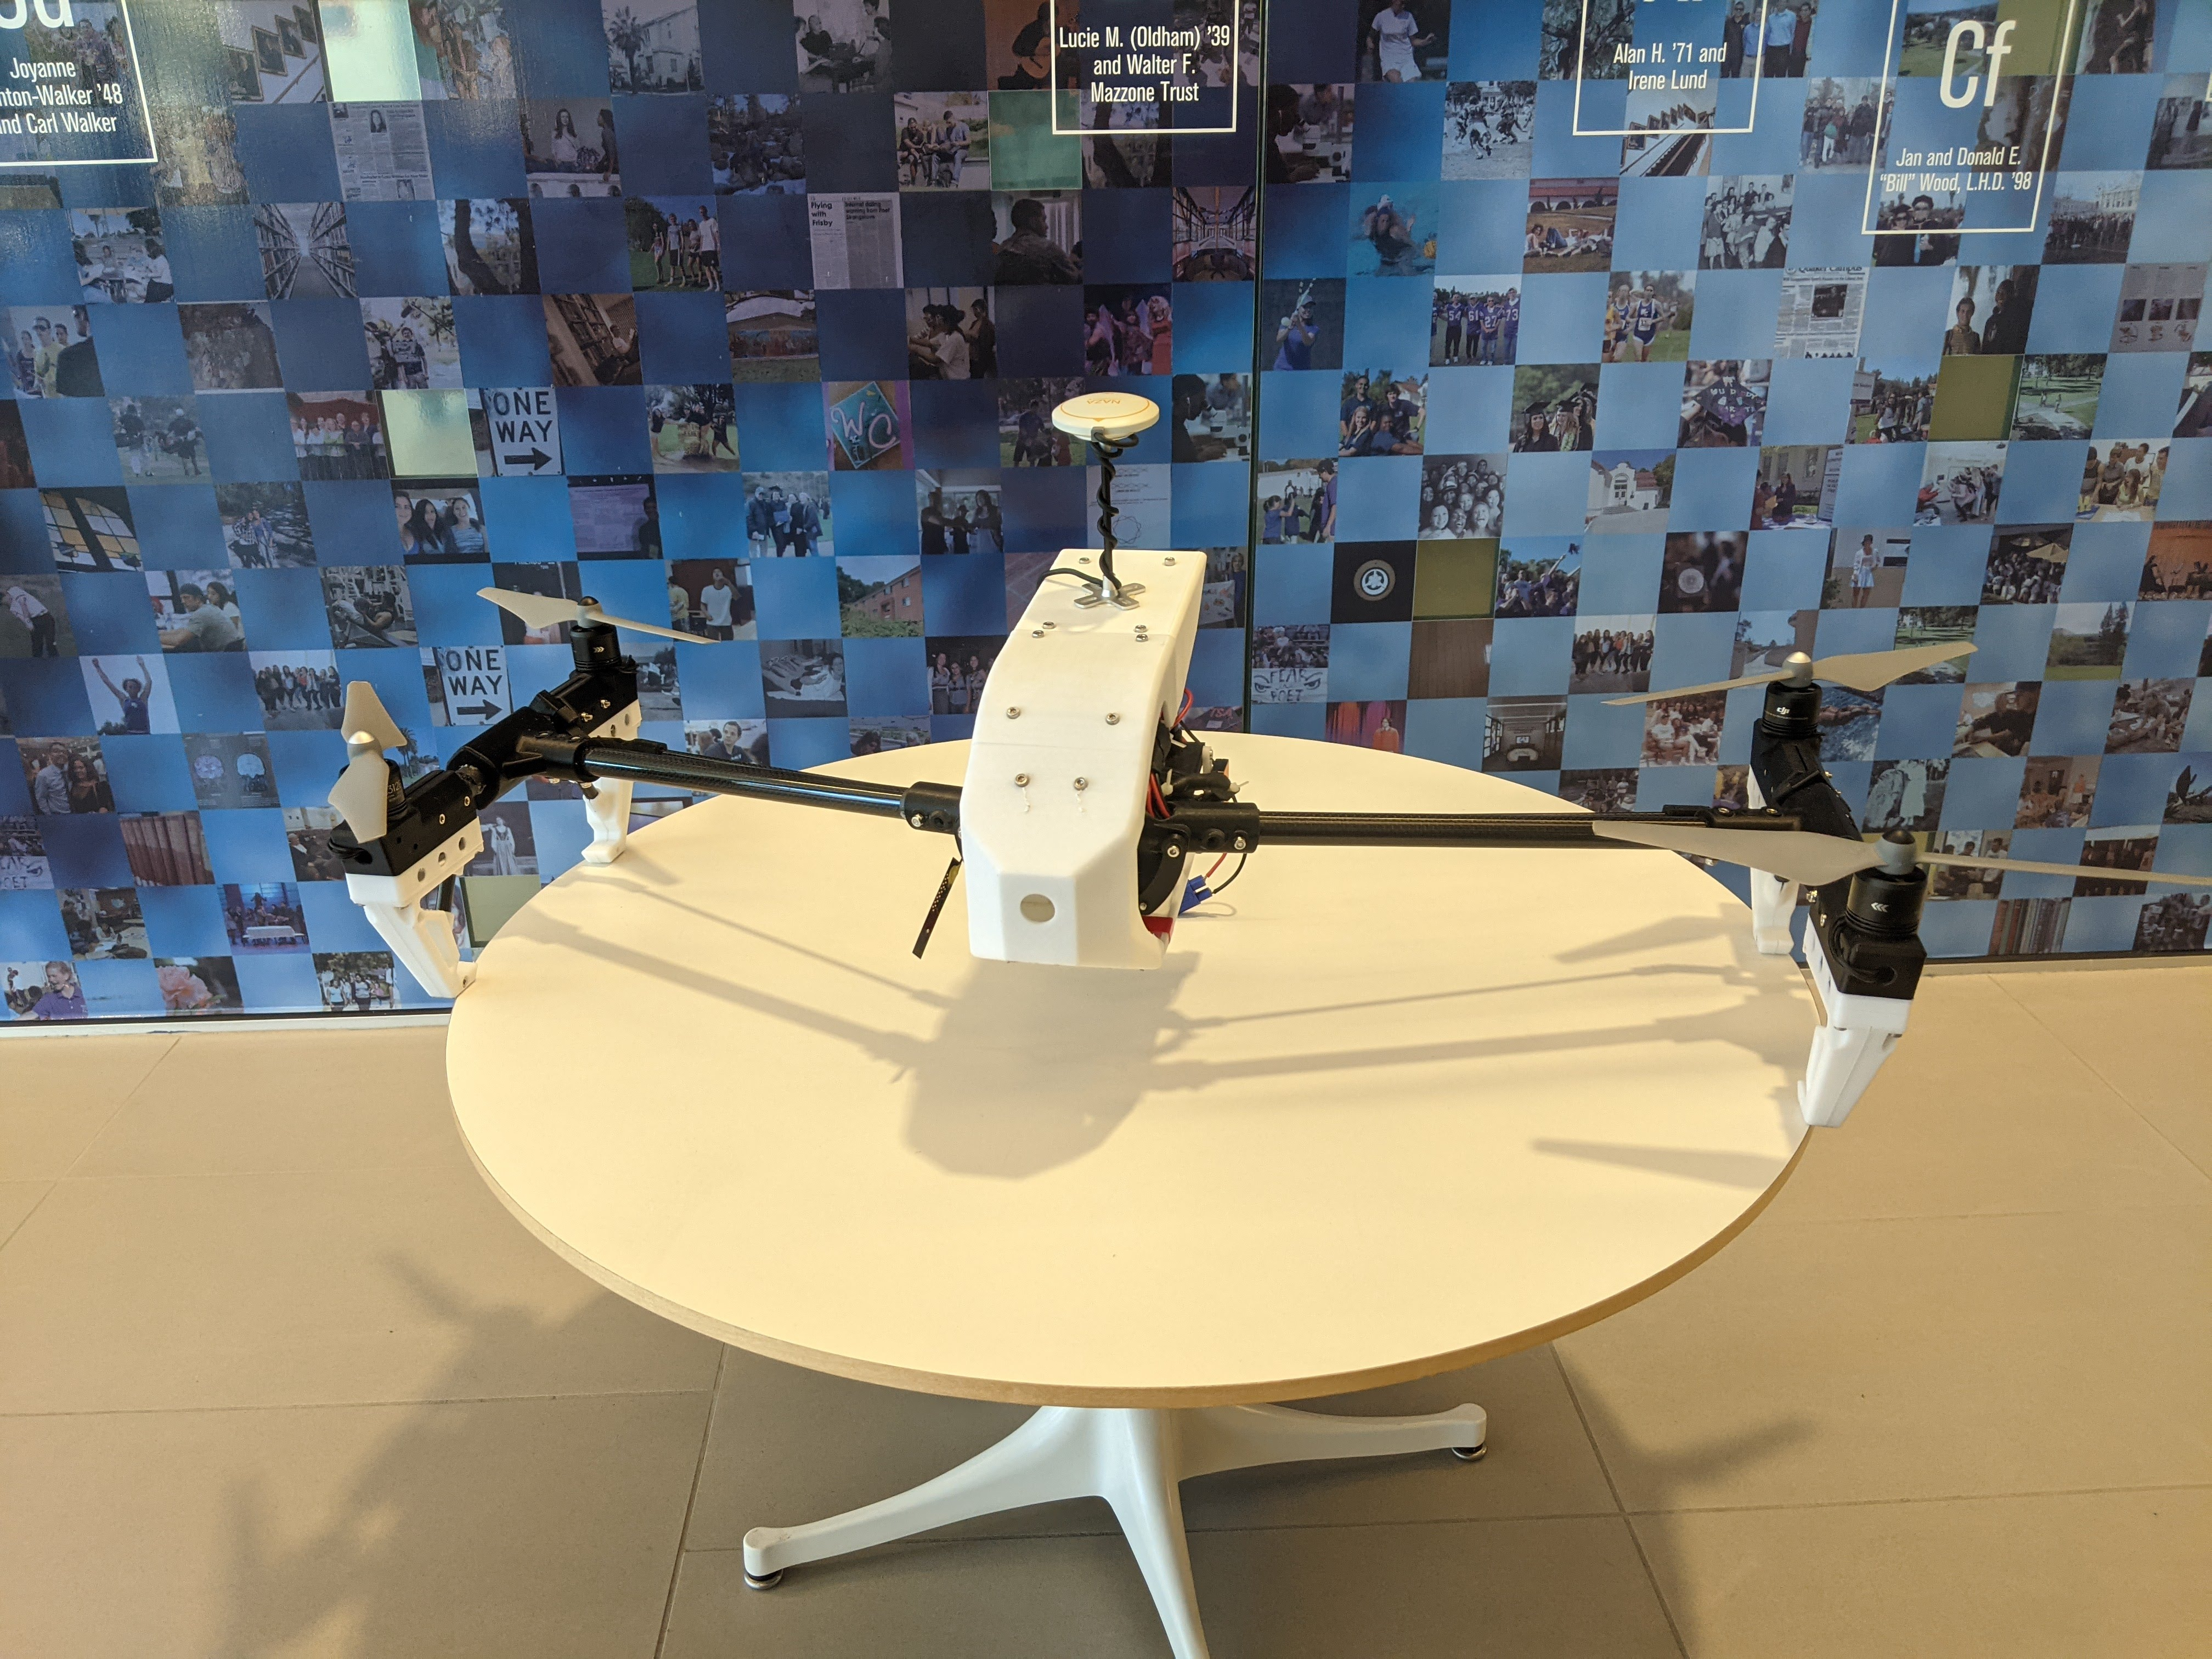
\includegraphics[width=0.6\textwidth]{drone.jpg}
\caption{\label{fig:drone} Our 3D-printed quad-rotor drone, designed and assembled by Whittier College undergraduates using our RF design lab and machine shop.  The unit is equipped with hand-held RC control, and GPS with programmable waypoints.}
\end{figure}

The incorporation of phased array radio sounding systems on UAS faces an optimization problem: the right balance between craft weight, thrust, payload, and flight time must be achieved.  To collect quality radio sounding data, the payload must be flown horizontally for $1-10$ km, implying $\approx 1$ hr battery life at reasonable speeds.  The requirement for longer flight times drives up battery size.  Increased battery size increases weight, which tends to decrease flight time.  Phased array payloads with a large number of elements could benefit data collection, but increased payload adds weight and decreases flight time.  The optimization is made far easier if the radar transmitter and receiver system is integrated into the hull of the UAS.  We propose to study how the RF phased array can be printed into the hull of the UAS, using machine learning to optimize beam-forming for radio sounding.  The Electrifi filament has a similar density to aluminum, meaning it can serve as \textit{both} a structural component and a phased array material.  Manufacturing structural components as phased array elements reduces costs, weight, and payload.  Through this research, we seek to advance the ongoing CReSIS effort to minimize radar units for UAS integration.  \\ \vspace{2.5mm}

As part of this engineering effort, we also propose to simulate expected results using MEEP.  Performing a CEM simulation that incorporates our current knowledge of ice properties with the UAS radar response would enrich the research in two ways.  First, such simulations enhance the design process, revealing design requirements, shortcomings, and ways to overcome them.  MEEP simulations require the user to specify the complex matrix for the dielectric constant of the medium, $\epsilon(x,y,z)$.  The $\epsilon$ matrix  determines how RF waves reflect, refract, and propagate back to the receiver.  Optimizing UAS phased array design for maximal $\epsilon(x,y,z)$ precision will result in optimal precision for $\lambda(x,y,z)$.  For dielectric materials, $\epsilon$ and $\lambda$ are related analytically \cite{10.3189/2015jog14j214}.  Second, building such MEEP simulations will provide a cross-check between the observed $\epsilon(x,y,z)$ from field data, and the simulated $\epsilon(x,y,z)$. \\ \vspace{2.5mm}

FDTD simulations are notorious for consuming computational resources like volatile memory, while providing the necessary resolution for $\epsilon(x,y,z)$, and electromagnetic fields versus time, frequency, and space.  At Whittier College, we have acquired a System76 Helio desktop system with AMD Ryzen threadripper 3990x 64-core, 128 thread processor.  The system has 0.5 GB of volatile memory per thread.  We have already shown that running MEEP in parallel on our system reduces run times by an order of magnitude \cite{meepcon2022}.  The reduction is due primarily to increased set up speed for $\epsilon(x,y,z)$.  Thus, we are already in a position to perform such CEM simulations quickly and efficiently.  Learning how to introduce parallelism into CEM problems will also be of educational benefit to our STEM undergraduates at Whittier College.

\section{Integration of Research and Education at Whittier College}
\label{sec:int}

The integration of CEM and additive manufacturing into our STEM curriculum will benefit our diverse undergraduates in two ways.  The first benefit is learning gains and boosted engagement from integrating our research into existing courses.  The second benefit will be the creation of undergraduate research opportunities.  For course integrations, there are some that can be done within our Department of Physics and Astronomy, and others that can take place in the Department of Mathematics and Computer Science.  We already have mathematics and computer science faculty at Whittier College who specialize in machine learning.  For example, Prof. Fred Park specializes in the application of machine learning and parallel computing to computer vision and image analysis \cite{SHI201528,doi:10.1137/20M1337041}.  We will work with those colleagues to integrate this research into courses like Computer Logic and Digital Circuit Design, Digital Signal Processing, Machine Learning, and Introduction to Data Science with Python.  I personally teach two of these courses, and I note below when collaboration with another instructor is required.  For undergraduate research opportunities, we already have a track record of success.  Our undergraduate researchers have made wonderful achievements in CEM, firmware design, and theoretical physics with our local Ondrasik-Groce and Fletcher Jones Fellowships.  Our goal is to expand this practice through NSF-sponsored research fellowhips in additive manufacturing, CEM, and machine learning.\\ \vspace{2.5mm}

%1. Course integrations for computational physics, electromagnetism, data science (COSC180 - Glenn)
%What courses exist that can be enhanced?  Jupyter as a learning mechanic
%2. Course integrations for machine learning and additive manufacturing
%Do we need a new course here?  Or just the math ones?  How can we merge additive manufacturing into a course
%3. What type of undergraduate research fellowship is appropriate?  Summers are the most productive.
%Highlight past funding and show that we can at least continue on that trajectory, and if it is enhanced, the
%project can succeed.

\subsection{Course Integrations - Electromagnetism and Computational Physics}
\label{sec:integration}

One straightforward set of course integrations that will take place within the Department of Physics and Astronomy are: Algebra-Based Physics II (Electricity, Magnetism, and Modern Physics), Calculus-based Physics II (Electromagnetism), Electromagnetic Theory, Optics, and Computational Physics\footnote{I personally teach Algebra-Based Physics II, Calculus-Based Physics II, and Electromagnetic Theory.  Optics and Computational Physics are normally taught by my colleagues within Physics and Astronomy.  Computational Physics will soon be handed to myself and others as the usual instructor retires.}.  The first two courses contain the standard introductory level course content on electromagnetism.  Simple web-based learning modules can be developed to illustrate the concepts of electromagnetic waves and optics via MEEP in Jupyter notebooks.  Jupyter (\url{https://jupyter.org/}) is an open-source project that supports interactive data science and scientific computing across all programming languages.  We have experience creating and sharing MEEP notebooks to accomplish research \cite{electronics10040415}, and in teaching Computer Logic and Digital Circuit Design using the PYNQ-Z1 SoC (\url{http://www.pynq.io/}). Such notebooks and modules can be integrated into Moodle, our web-based content management system (CMS).  The primary enhancement to student learning is to illustrate dynamic electromagnetic fields subject to interesting boundary conditions.  These examples should be shown alongside similar textbook examples, so the students can compare them.  The final projects are student-designed DIY physics experiments in DC circuits, optics, and magnetism.  We look forward to introductory students who accept the challenge of matching simulation output to their real-world results. \\ \vspace{2.5mm}

As part of our tenure-track process, we at Whittier College are required to submit reflective analyses of our teaching, research, service, and advising every two years.  The teaching reflections have revealed the learning value of the synergies between traditional lecture content, simulations, and lab experiments.  Students in Algebra-Based and Calculus-Based Physics are fully prepared to apply ideas of physics in their own projects when the ideas solidify in their minds.  Solidification occurs when they demonstrate them as theoretical predictions, simulate them, and test them in the lab.  After solidification, their confidence is such that they stop questioning their understanding of a concept and start to use it.  A good example is DC circuit analysis.  We first solve systems of equations that predict currents through multiple devices connected to a battery.  In a popular PhET simulation, PhET DC Circuit Construction Kit, current and charge are animated, and students can make virtual (simluated) measurements.  The students replicate the virtual circuit in the lab, and show that the volts and amps in real life match the simulation.  Apprehension fades to confidence when they see that they got it all to match.  There are few HTML5 PhET simulations that illustrate dynamic electromagnetic fields.  We can use Jupyter modules with MEEP to fill this gap. \\ \vspace{2.5mm}

We have three opportunities to integrate this research within advanced physics courses: Optics, Electromagnetic Theory, and Computational Physics.  Our Optics course introduces students to three areas.  The first is ray optics, with discussions of lenses and optical instruments.  The second is wave optics, with discussions of superposition, interferance, and diffraction. The third is modern optics, with discussions of photons, spectra, lasers, interferometry, fiber optics, and nonlinear optics.  One useful module in ray optics would be a lens example that demonstrates magnification of images and focal length.  As the course progresses to wave optics, the lens example could be enhanced more more complex, photonics examples \cite{meepcon2022_3}.  The modern optics curricula presents rich opportunities to demonstrate course concepts, including flux and spectral monitoring for diffraction gratings \cite{meepcon2022_4}, and waveguides for fiber optics \cite{meepcon2022_5}.  These modules will prove useful to our students, because most Optics students have had at least one semester of Python (Computer Science 1) and one semester of Modern Physics.  As I do not personally teach this course, the adoption of these modules can be at the discretion of the normal instructor.  Our department is small (four faculty), and has a good track record of collaboration.  \\ \vspace{2.5mm}

The course integration in Electromagnetic Theory carries great potential.  This one-semester course usually covers chapters 1-7 of \textit{Introduction to Electrodynamics} by D. Griffiths (Cambridge University Press, 2017), with some examples of electromagnetic waves.  Though students are exposed to electromagnetic waves in an intermediate course (Modern Physics), the advanced course gives a minor elaboration on waves in vacuum.  Using Jupyter modules with CEM, students can be exposed to the interaction of waves with non-uniform dielectric media.  The difference between ray-tracing and true three-dimensional propagation in polar ice with $n(x,y,z)$ is an excellent example of how the UHE-$\nu$ research, CEM, and teaching all coalesce (see Sec. \ref{sec:askaryan}).  Another possibility is to introduce waveguides and related devices.  There are many examples in the MEEP documentation, including ``the S-parameters of a directional coupler.''  It was this example that provided the open-source code for computing the S-parameters of our RF antenna designs \cite{meepcon2022}.  Finally, we can introduce a Jupyter module encompassing specular and diffuse reflection from rough surfaces.  This module would connect the CReSIS radio sounding research, CEM, and teaching together (see Sec. \ref{sec:cresis}).  Once the 3D printed RF antennas are produced, they can be showcased as a practical application of electromagnetic theory and CEM.  \\ \vspace{2.5mm}

\subsection{Course Integrations - Computer Logic and Digital Circuit Design, and Digital Signal Processing}

As part of my teaching practice at Whittier College, I regularly create and teach computer science courses.  Among these are Computer Logic and Digital Circuit Design, and Digital Signal Processing.  The former covers number systems, Boolean algebra and complex logic functions, adders, encoders, comparators, shift-registers and memory, counters, finite state machines, timing diagrams, firmware programming with Python, and lab techniques for digital circuits, and ADC/DAC.  The laboratory component of this course is performed on the PYNQ-Z1 SoC (\url{http://www.pynq.io/}), allowing students to write firmware in Python.  Examples of laboratory activities in this course include creating digital logic functions with LED outputs and ADC/DAC examples with Digilent PMODs.  There are a plethora of examples with the PYNQ community that demonstrate neural networks and image/video processing that all involve some form of FPGA acceleration.  These examples can serve as inspiration for algorithms that will aid in the CEM design phase for the phased array research.  Many of the students who take this course will be actively seeking research opportunities, and we have recruited research students from this course in the past.  Thus, boosting the machine learning and FPGA acceleration aspects of the course will serve educational and research purposes. \\ \vspace{2.5mm}

Digital Signal Processing (DSP) is another course I created and teach reguarly within Computer Science.  Among the topics covered are statistics and probability, complex numbers, noise in digital systems, ADC/DAC, sampling and digitization, Fourier series, Fourier and discrete Fourier transforms (DFTs), Laplace and z-transforms, linear time-invariant (LTI) systems and filtering, audio and image processing, applications to digital circuits, and applications of neural networks.  Though this course was originally created independently of Computer Logic and Digital Circuit Design, it has evolved to become a continuation of it.  These two courses can take students all the way from basic binary to complex analysis of digitized signals.  A potential course integration between DSP and our open-source CEM research is the application of DFTs to MEEP flux monitors and near-to-far-field monitors.  These are CEM objects that compute the integrated flux of radiation passing through a surface as a function of frequency using a DFT.  Students can see that the radiation is nothing more than a digitized sampled signal within a CEM context, and that the DFT is a tool for understanding the radiation spectrum.  We can adapt Jupyter modules we have already written to this task. \\ \vspace{2.5mm}

\subsection{Course Integrations - Introduction to Data Science with Python, and Machine Learning}

Two additional courses within the Mathematics and Computer Science Department that represent integration opportunities are Introduction to Data Science with Python, and Machine Learning.  The former is an introductory course that assumes the student has basic programming skills.  The students learn import, explore, analyze, and visualize data using tools like Jupyter notebooks, NumPy, and Matplotlib.  More advanced tools like Pandas, SciPy, and scikit-learn are introduced.  The inclusion of Jupyter notebooks that generate data sets using CEM into the syllabus is straightforward.  Quantities like radiation patterns and S-parameters versus frequency are fertile grounds for learning to visualize data with Matplotlib, as we have already done in publications \cite{electronics10040415}.  Since scikit-learn is already included in the syllabus, performing RF antenna optimization with machine learning tools within scikit is also straightforward.  Though I personally do not teach this course, it is taught by Prof. Glenn Piner, who is our colleague in the Department of Physics and Astronomy.  By working together to incorporate these ideas as appropriate into this introductory course, our students will gain early preparation to perform the cutting edge research with MEEP and additive manufacturing.  Ideally, once the RF antennas are manufactured, we can demonstrate their performance in class to provide the students with a real world application. \\ \vspace{2.5mm}

Our more advanced computer science course in this area is Machine Learning.  Typically taught by Prof. Fred Park, this course assumes a more advanced knowledge of Python and Calculus II.  Topics include unsupervised and supervised learning, data clustering, principle component analysis, logistic regression, support vector machines, neural networks, and deep learning.  One topic that might prove a useful addition to the list of topics is genetic programming, because this technique has been used to optimize RF antennas \cite{2016MsT.........58S,genetic}.  We will work together to incorporate genetic programming as appropriate into the syllabus.  As with Data Science, demonstrations of the optimized RF antenna would be ideal.  This integration should enhance the course, because students will see the practical application of technical ideas in the fields of physics and geophysics, and climate science.  This course in particular will be in high demand, because students understand the large number of opportunities that await them in the defense and software development sectors in Southern Californa once they master machine learning.  One such opportunity will be our newly created Educational Partnership Agreement (EPA) with NSWC Corona.  Our students will be doubly prepared for internships through the EPA, through the engineering experience from the RF application, and the machine learning training.

\section{Translation of STEM Research for our Community}
\label{sec:broad}

Our proposed project will provide valuable opportunities to diverse students from our community, which is heavily influenced by our bilingual families.  Families that speak Spanish at home and English at school are very common at Whittier College (an HSI).  For Fall 2022 admitted students, 36\% are Hispanic/Latino, and another 8\% are International students.  Over the past five years, students of color and first-generation students have comprised 69\% and 34\% of the student body, respectively.  We have observed that students of color receive lower grades than their peers in our introductory STEM courses (see Tab. \ref{tab:grades}).  We have learned from workshops that emphasizing the dignity and self-efficacy of the student works againts disparity \cite{cottrell1,cottrell2}.  In keeping with the project theme of \textit{translation} of progress in one area to serve another, and in order to emphasize the dignity of our students no matter their background or the adversity they encounter, we seek to produce a bilingual mobile application introducing STEM concepts within a welcoming digital environment. \\ \vspace{2.5mm}

\begin{table}
\centering
\begin{tabular}{c c c c}
Discipline & GPA (Students of Color) & GPA (White) & Shift \\ \hline
Physics & 2.62 & 3.15 & -0.53 \\
Mathematics & 2.54 & 2.75 & -0.21 \\
Computer Science & 2.77 & 3.31 & -0.54 \\
Chemistry & 3.02 & 3.20 & -0.18 \\
Biology & 3.03 & 3.18 & -0.15 \\
Environmental Science & 3.17 & 3.25 & -0.08 \\
\end{tabular}
\caption{\label{tab:grades} GPA data for Whittier College students from Fall 2016 to Spring 2021, disaggregated by racial background and discipline.  See text for details.}
\vspace{-0.5cm}
\end{table}

Implementation of the Duolingo method for language and mathematics on a mass scale has provided promising results \cite{duolingo_whitepaper}.  Results presented within the educational data mining (EDM) literature provides additional examples of apps and techniques that boost engagement and success in introductory STEM courses \cite{edm1,edm2,edm3,edm4}.  Some members of our community have shared that translating mathematics and physics exercises into Spanish aids in solving them.  Our app will boost their skills and build confidence by offering them engaging, game-like physics training in the language of their choice.  Even if the base language of STEM content in our courses does not represent a barrier for our students, the design of our app, based on the Duolingo Method, should boost the skill of all our students. \\ \vspace{2.5mm}

The Duolingo method has five main components \cite{duolingo_whitepaper}.  The first component is Learning by Doing, or utilizing the innate learning toolkit every student has.  Learning by doing also involves affordance-based design, embodied cognition, and explicit instruction.  The second component is to Learn in a Personalized Way.  This involves utilizing machine learning to ensure content is just difficult enough for the individual student to grow, but not so difficult that the student becomes disengaged.  The distinction hinges on ``desirable'' difficulty, versus ``undesirable'' difficulty.  The third component is to Focus on What Matters.  This component is about ensuring course content is matched to verified learning standards like Common Core.  The fourth component is to Stay Motivated.  Using game-like design with points, rewards, leaderboards, and collaboration has been shown to motivate students in a positive way.  The fifth is to Feel the Delight. This component is many things: quality storytelling, including diverse characters within the app, and providing moral encouragement.  The key is to create a positive environment conducive to learning.  \\ \vspace{2.5mm}

Two additional themes are relevant for mathematics learning in the Duolingo method: using multiple mathematical representations for the same concept (see Sec. \ref{sec:integration}), and the manipulation of tools.  Both themes follow the concrete-real-abstract (CRA) learning progression.  A CRA progression is used to guide students towards understanding abstract mathematical concepts by first introducing them with concrete tools or representations, and gradually increasing the level of abstraction.  According to the authors, ``Equations, pictures, and narratives can all be used to describe mathematical concepts.  Moreover, using multiple representations supports learners' analogical thinking abilities ... Because these representations also are at varying levels of abstraction, we construct lessons so learners experience representations which are closer to real objects before they interact with more abstract representations'' \cite{duolingo_whitepaper}. \\ \vspace{2.5mm}

Once implemented, we have two goals for the app.  First, we seek to test the \textit{hypotheses} that the Duolingo method, and the two additional math themes, will boost the GPA results in Tab. \ref{tab:grades} and reduce disparities.  Second, we seek to affirm our students' dignity and cultural identity by making the app bilingual.  We hope these twin goals will serve to build confidence in our students by welcoming them into STEM learning at the college level. \\ \vspace{2.5mm}

\textbf{Educational Application for Student Learning of STEM (EASTLOS)}.  A prototype application, code-named EASTLOS for ``East Los Angeles'' (our geo-cultural area) is being built by Whittier College undergraduates.  The software and digital design of the app represents an opportunity for Whittier College students to enhance the learning experience for their peers while gaining valuable work experience.  In our budget and project planning we include paid student positions for code and digital design, and allocate time and space to finish the application.  By recruiting and using home-grown talent, we hope to inspire a passionate set of diverse software designers to help implement and disseminate the app.  We include three general phases in our project planning (Sec. \ref{sec:time_im}).  (1) We will desig and implement the app for an introductory physics course.  (2) We will use the app to gather data and make improvements.  (3) We will present results to a broader audience, and help to implement the app in other courses and in the wider community. \\ \vspace{2.5mm}

\section{Bilingual Public Lectures and Recruitment Events}

Example

\section{Timeline and Project Planning}
\label{sec:time_im}

An example figure.

\begin{figure}
\centering
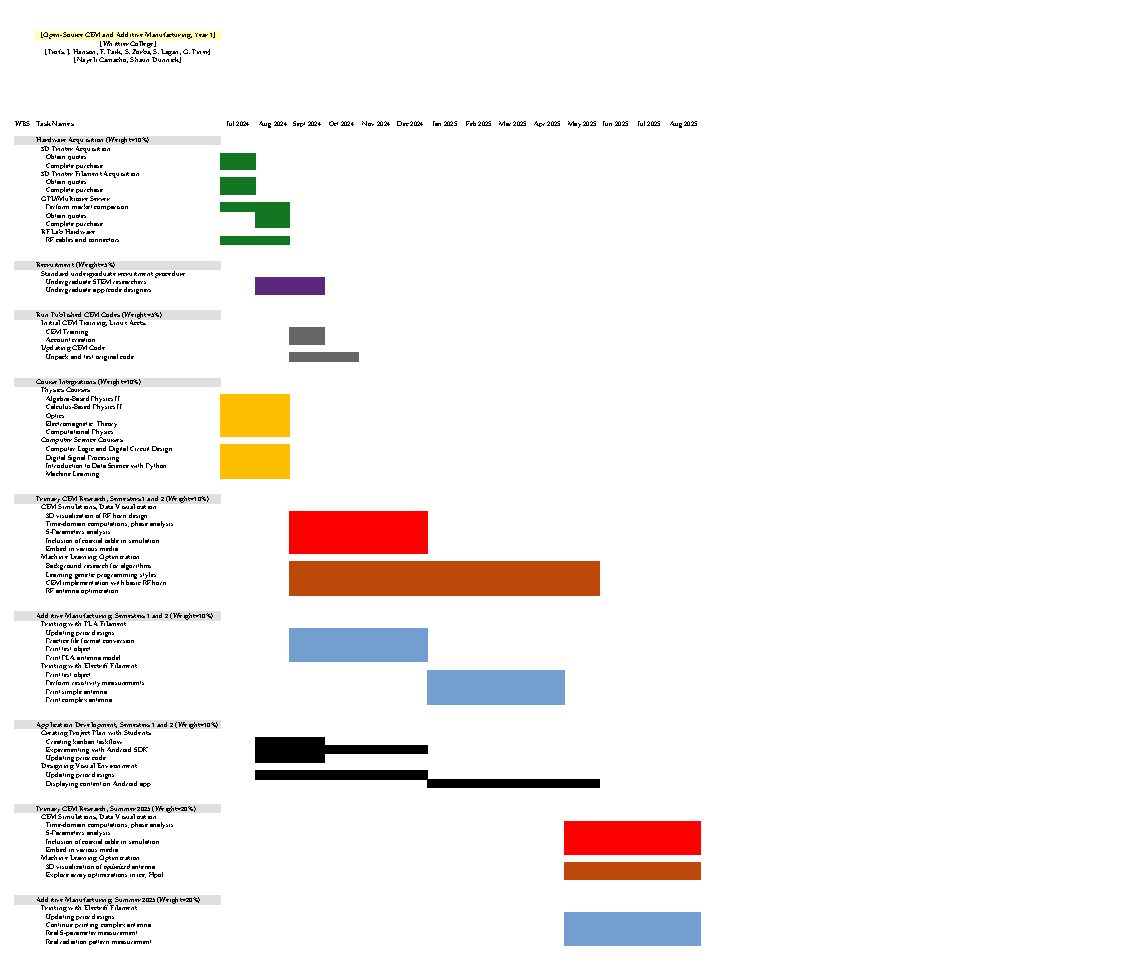
\includegraphics[width=0.99\textwidth,trim=0cm 0cm 6.5cm 0cm,clip=true]{project_planning/cem_project_gantt_year_1a.pdf}
\caption{\label{fig:gantt_1a} A Gantt chart outlining project planning, in visual form, for Year 1 of the project.}
\end{figure}

\begin{figure}
\centering
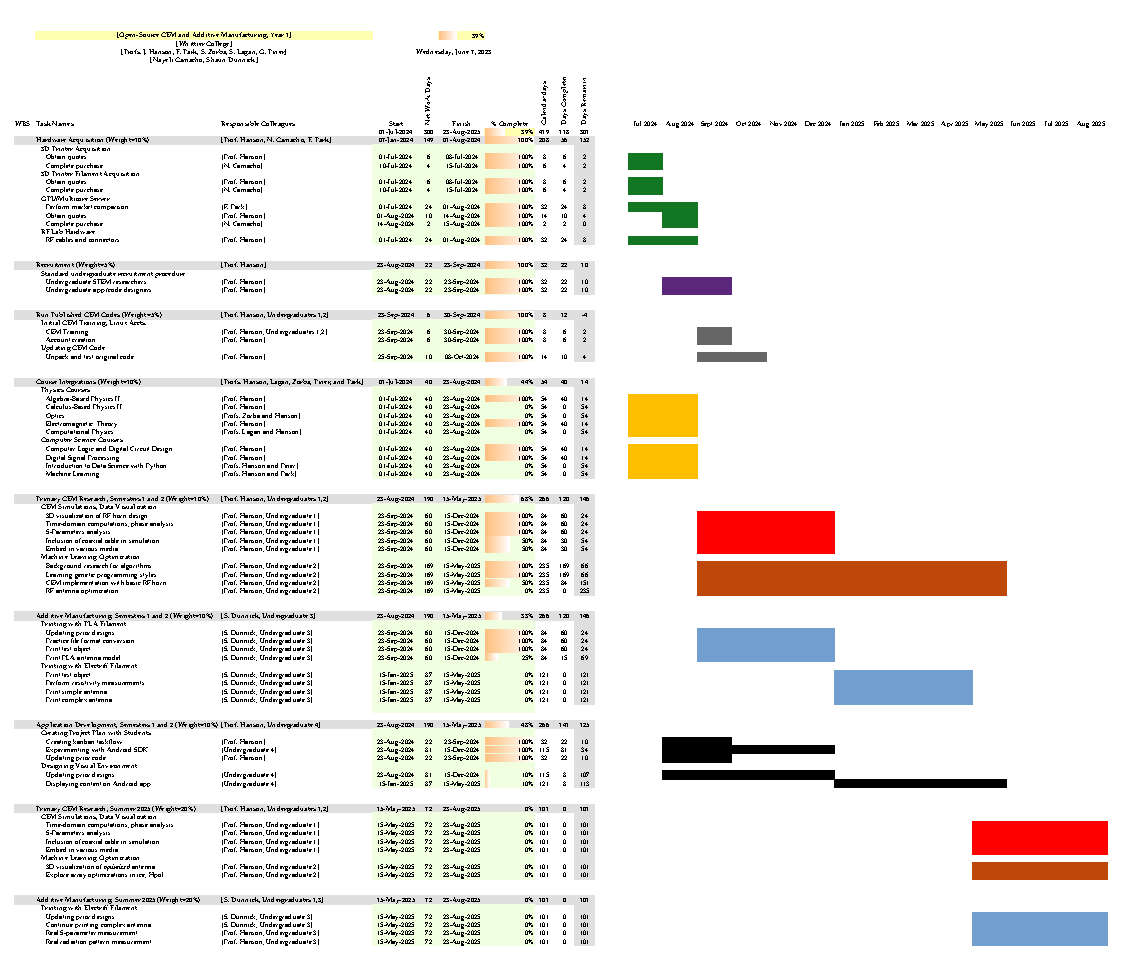
\includegraphics[width=0.99\textwidth,trim=0cm 8.25cm 9cm 0cm,clip=true]{project_planning/cem_project_gantt_year_1.pdf}
\caption{\label{fig:gantt_1b} A Gantt chart outlining project planning, in numerical form, for Year 1 of the project (part 1).}
\end{figure}

\begin{figure}
\centering
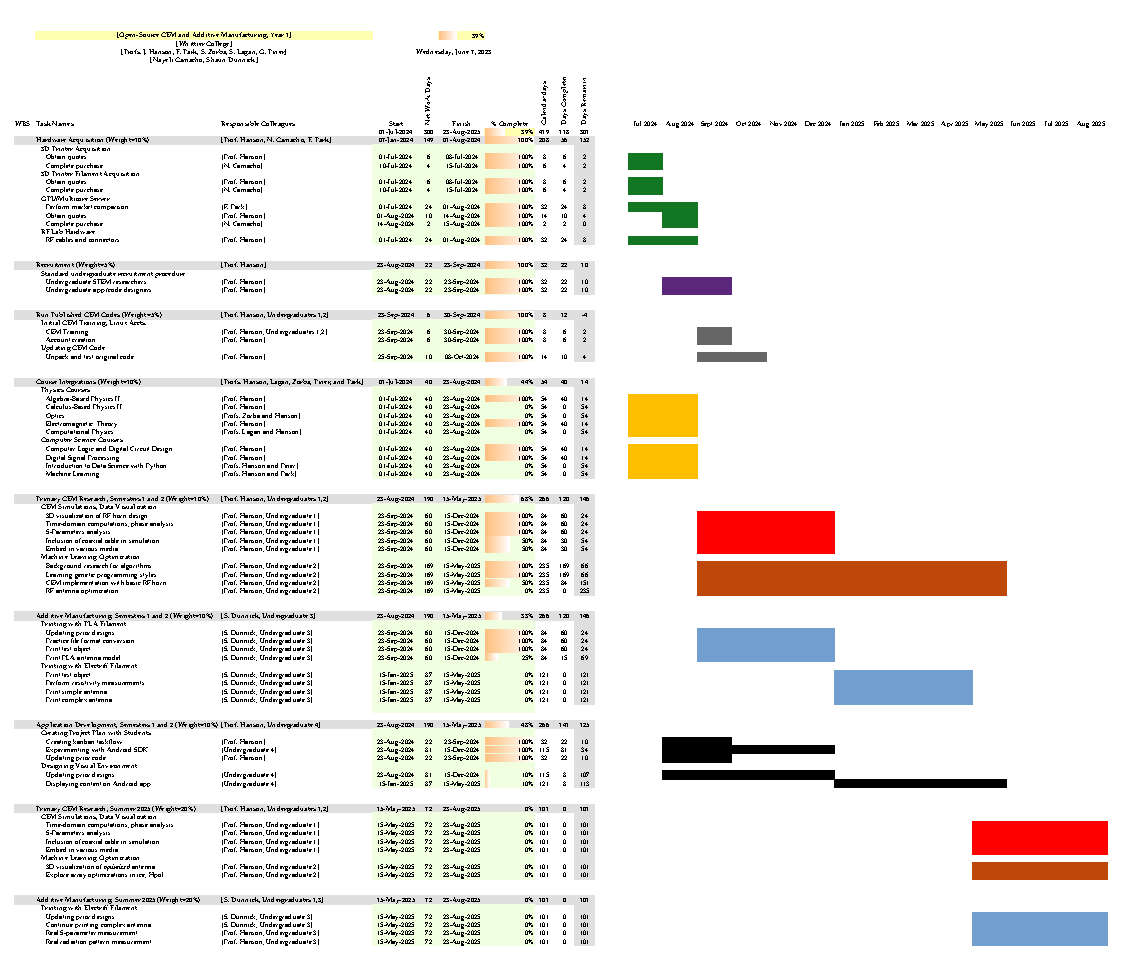
\includegraphics[width=0.99\textwidth,trim=0cm 0cm 9cm 8.25cm,clip=true]{project_planning/cem_project_gantt_year_1.pdf}
\caption{\label{fig:gantt_1c} A Gantt chart outlining project planning, in numerical form, for Year 1 of the project (part 2).}
\end{figure}

\end{document}
